\section{Supplementary figures}


\begin{suppfigure}[H]
\centering
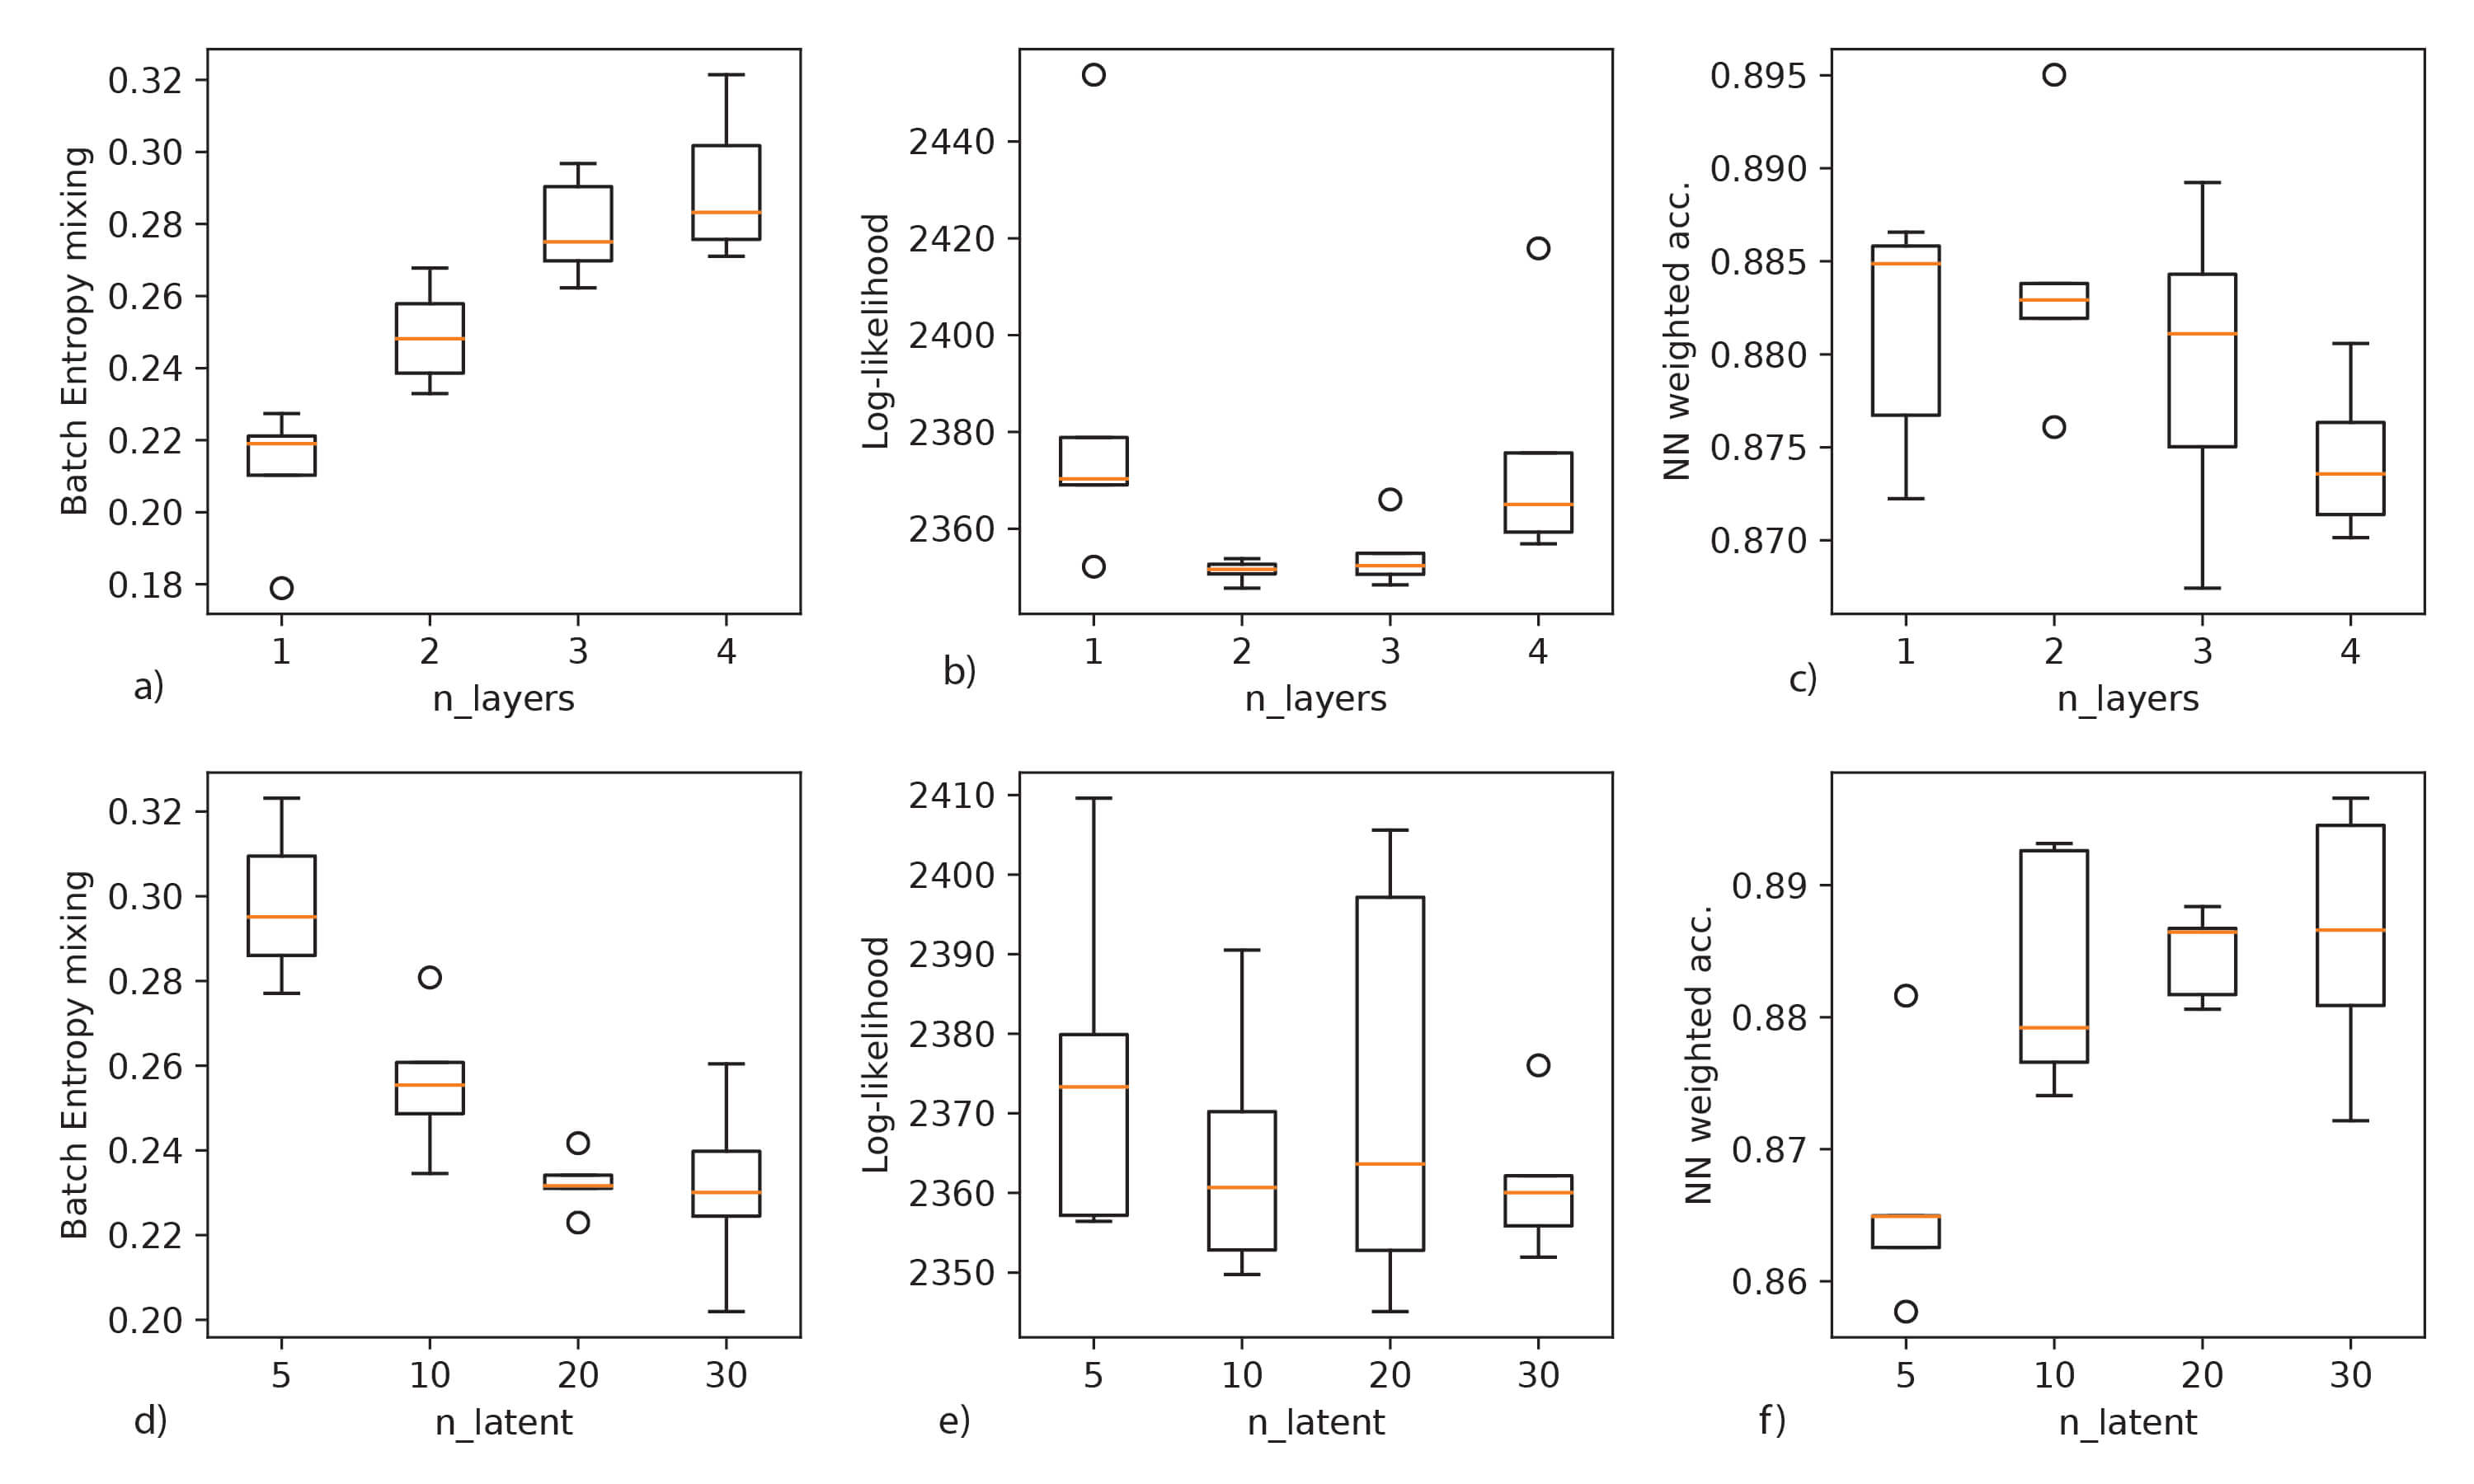
\includegraphics[width=\textwidth]{figures/robust.jpg}
\caption[Robustness analysis for harmonization of the pair of datasets MarrowMT-10x / MarrowMT-ss2 with scVI]{Robustness analysis for harmonization of the pair of datasets MarrowMT-10x / MarrowMT-ss2 with scVI. $(a-c)$ We augment the number of hidden layers in the neural network $f_w$ and track across $n=5$ random initializations for the batch entropy mixing $(a)$, the held-out log likelihood $(b)$ and the weighted accuracy of a nearest neighbor classifier on the latent space $(c)$. $(d-f)$ We increase the number of dimensions for the latent variable $z$ and track across $n=5$ random initialization the batch entropy mixing $(d)$, the held-out log likelihood $(e)$ and the weighted accuracy of a nearest neighbor classifier on the latent space $(f)$.}
\label{scanvirobustness_supplement}
\end{suppfigure}

\begin{suppfigure}[H]
    \centering
    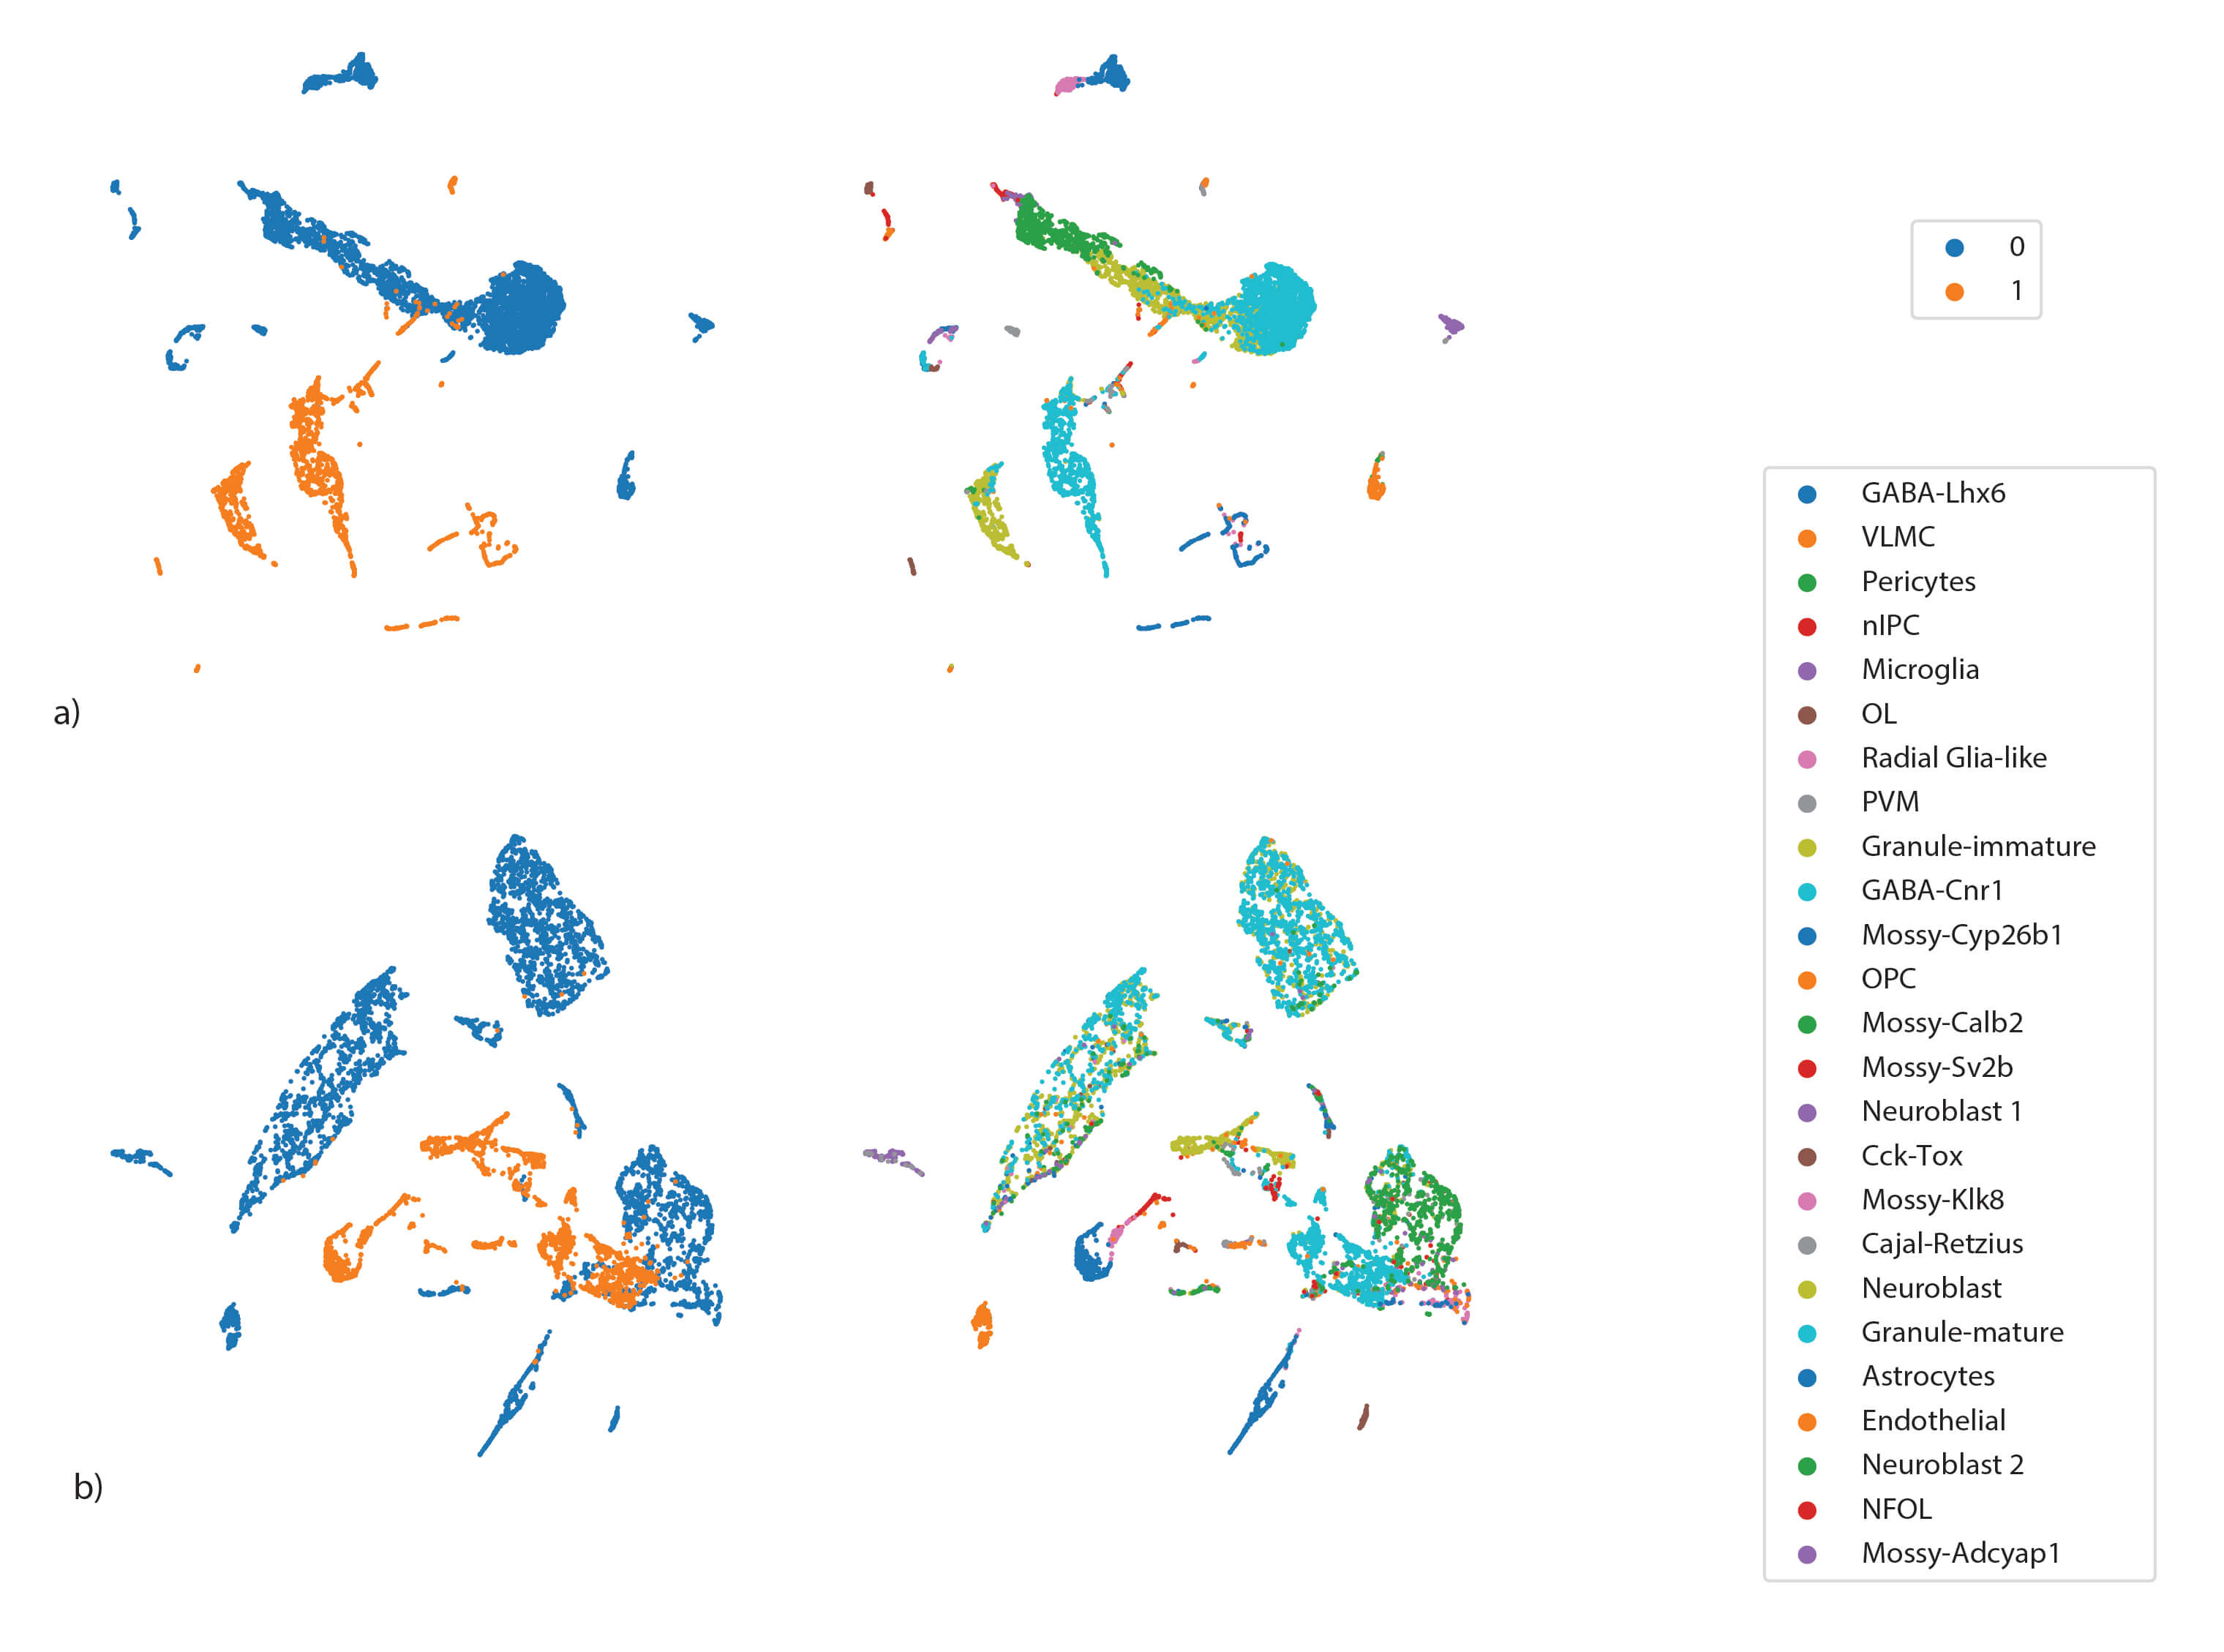
\includegraphics[width=\textwidth]{figures/magan.jpg}
    \caption[Visualization of the output of MAGAN on the DentateGyrus pair of datasets.]{Visualization of the output of MAGAN on the DentateGyrus pair of datasets. Using MAGAN, we projected the first dataset into the second one $(a)$ and vice-versa $(b)$. }
    \label{scanvimagan}
\end{suppfigure}

\begin{suppfigure}[H]
\centering
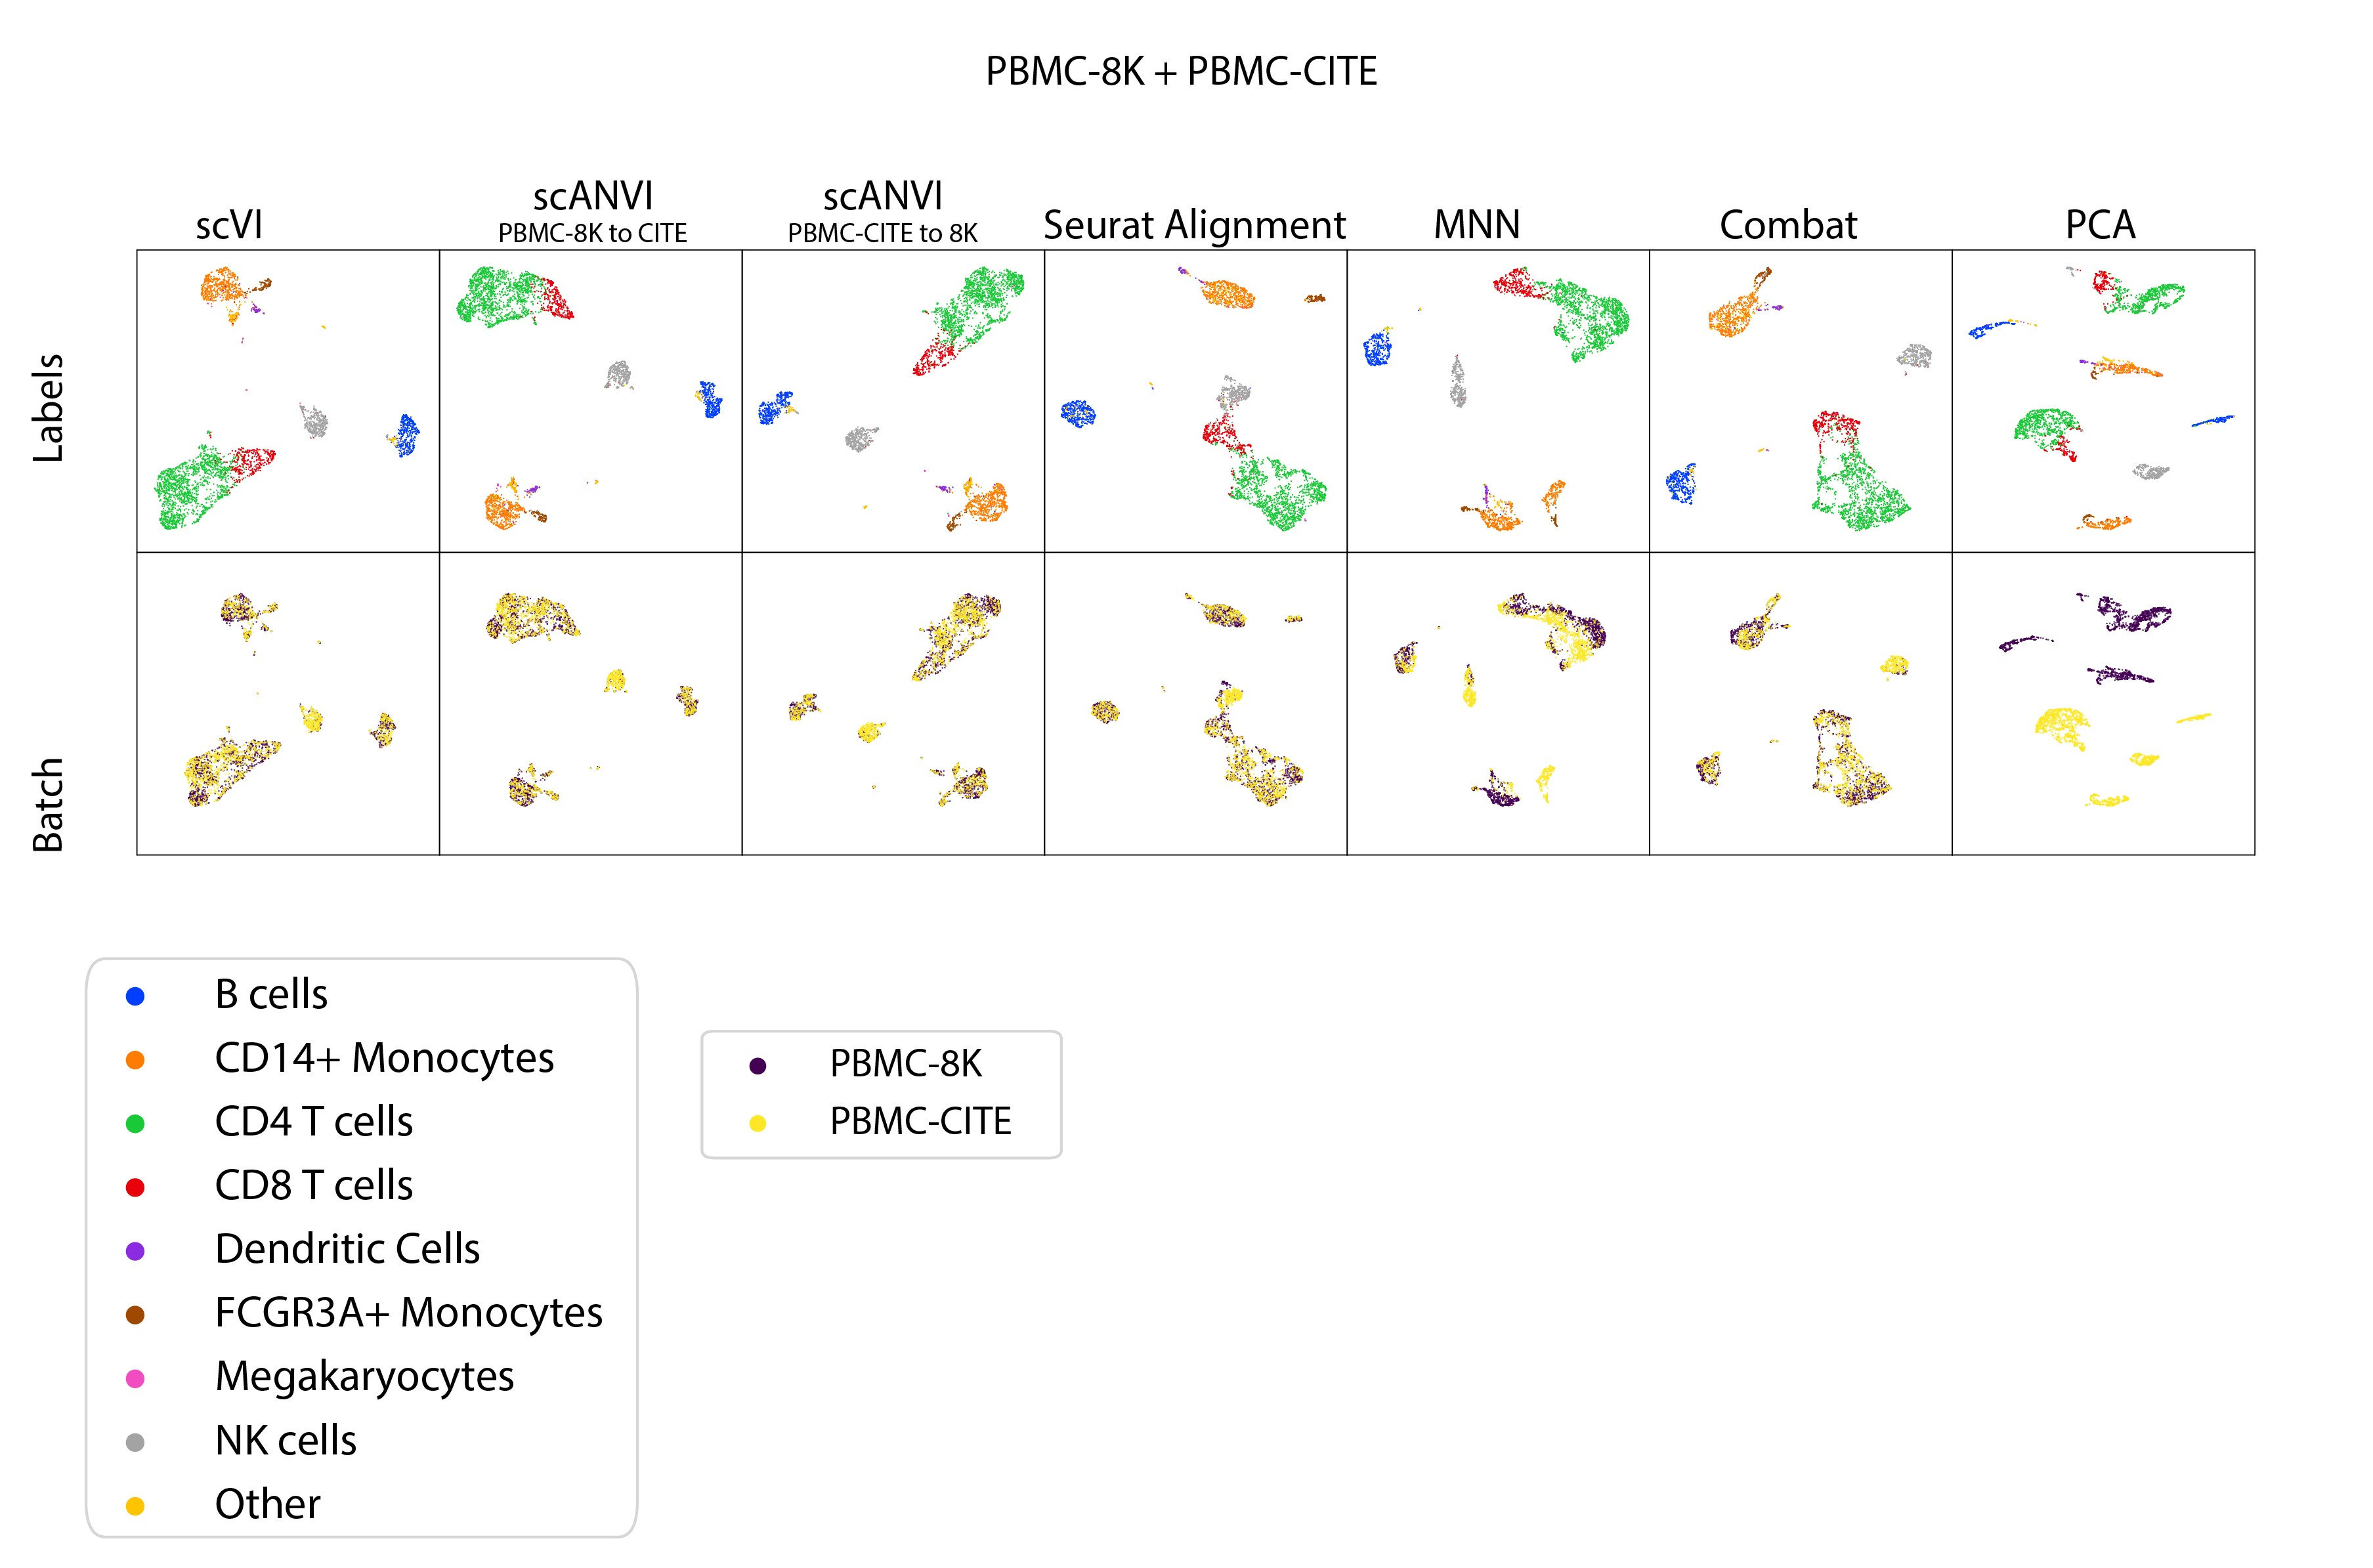
\includegraphics[width=\textwidth]{figures/supFig1-Easy1.jpg}
\caption[Visualization of the benchmark PBMC-8K / PBMC-CITE.]{Visualization of the benchmark PBMC-8K / PBMC-CITE. All positions for the scatter plots are derived using UMAP on the latent space of interest.}
\label{scanviEasy1}
\end{suppfigure}



\begin{suppfigure}[H]
\centering
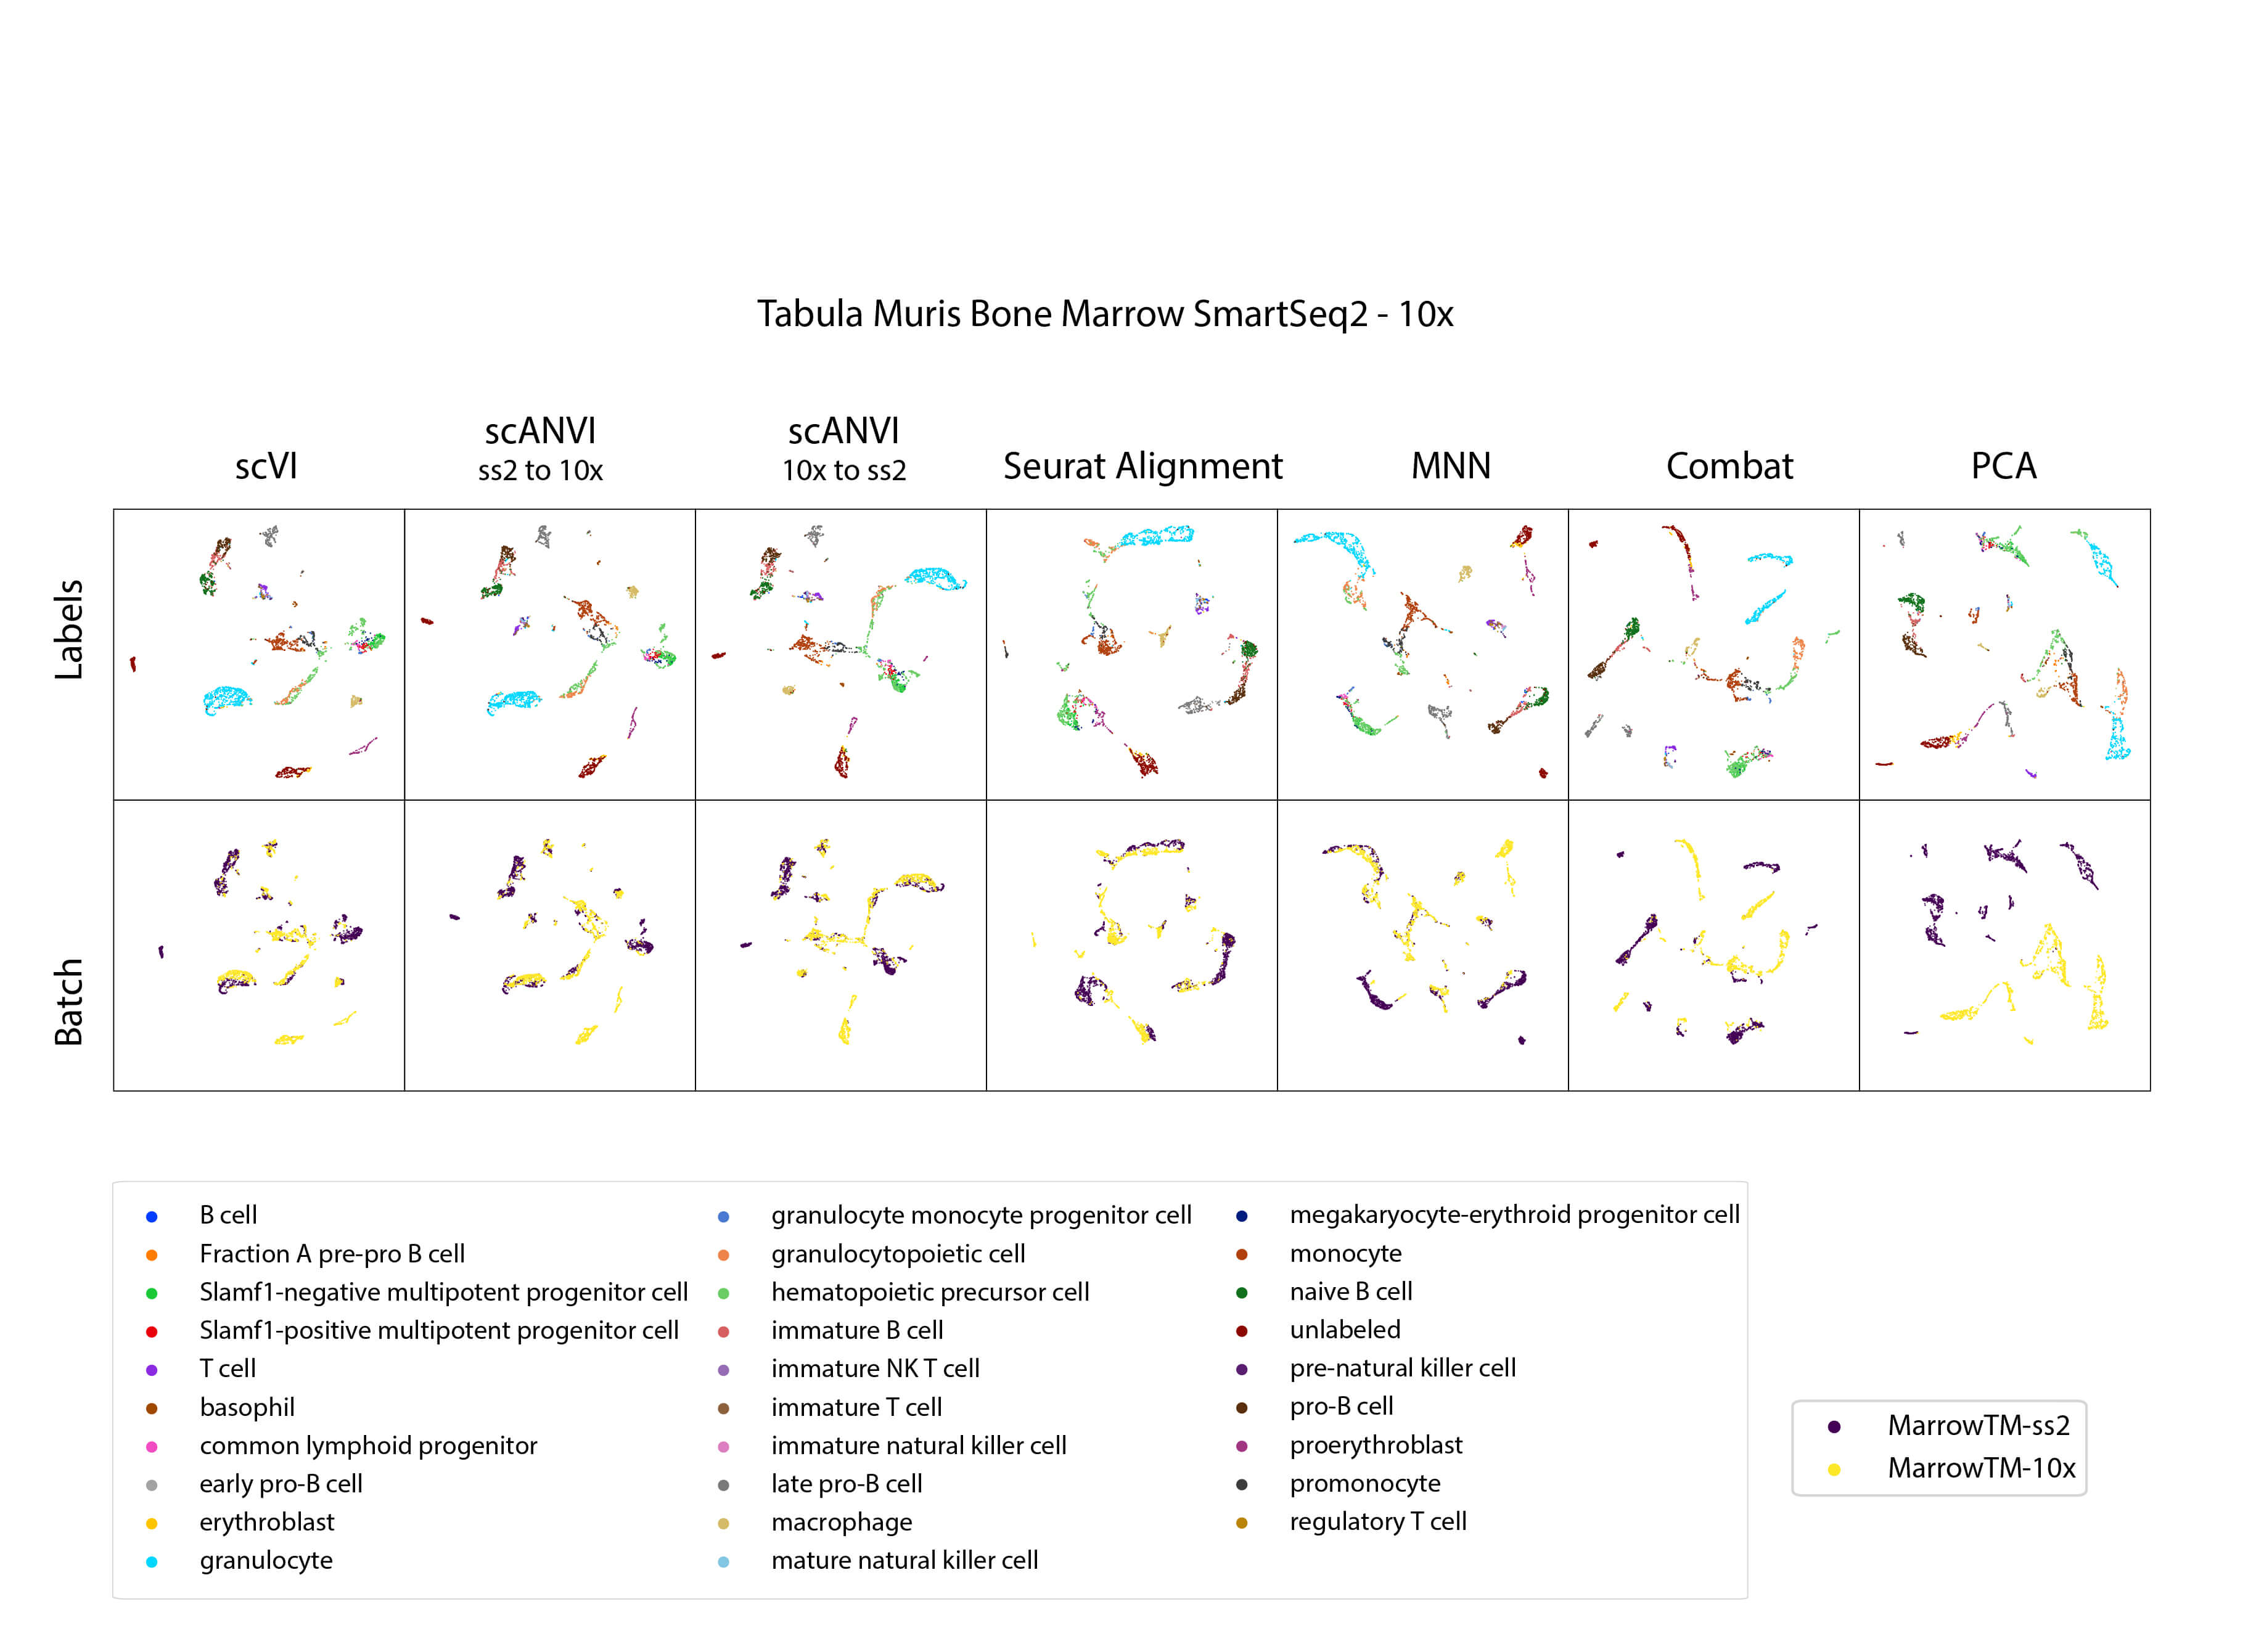
\includegraphics[width=\textwidth]{figures/supFig1-Tech1.jpg}
\caption[Visualization of the benchmark MarrowMT 10x / ss2.]{Visualization of the benchmark MarrowMT 10x / ss2. All positions for the scatter plots are derived using UMAP on the latent space of interest.}
\label{scanviTech1}
\end{suppfigure}


\begin{suppfigure}[H]
\centering
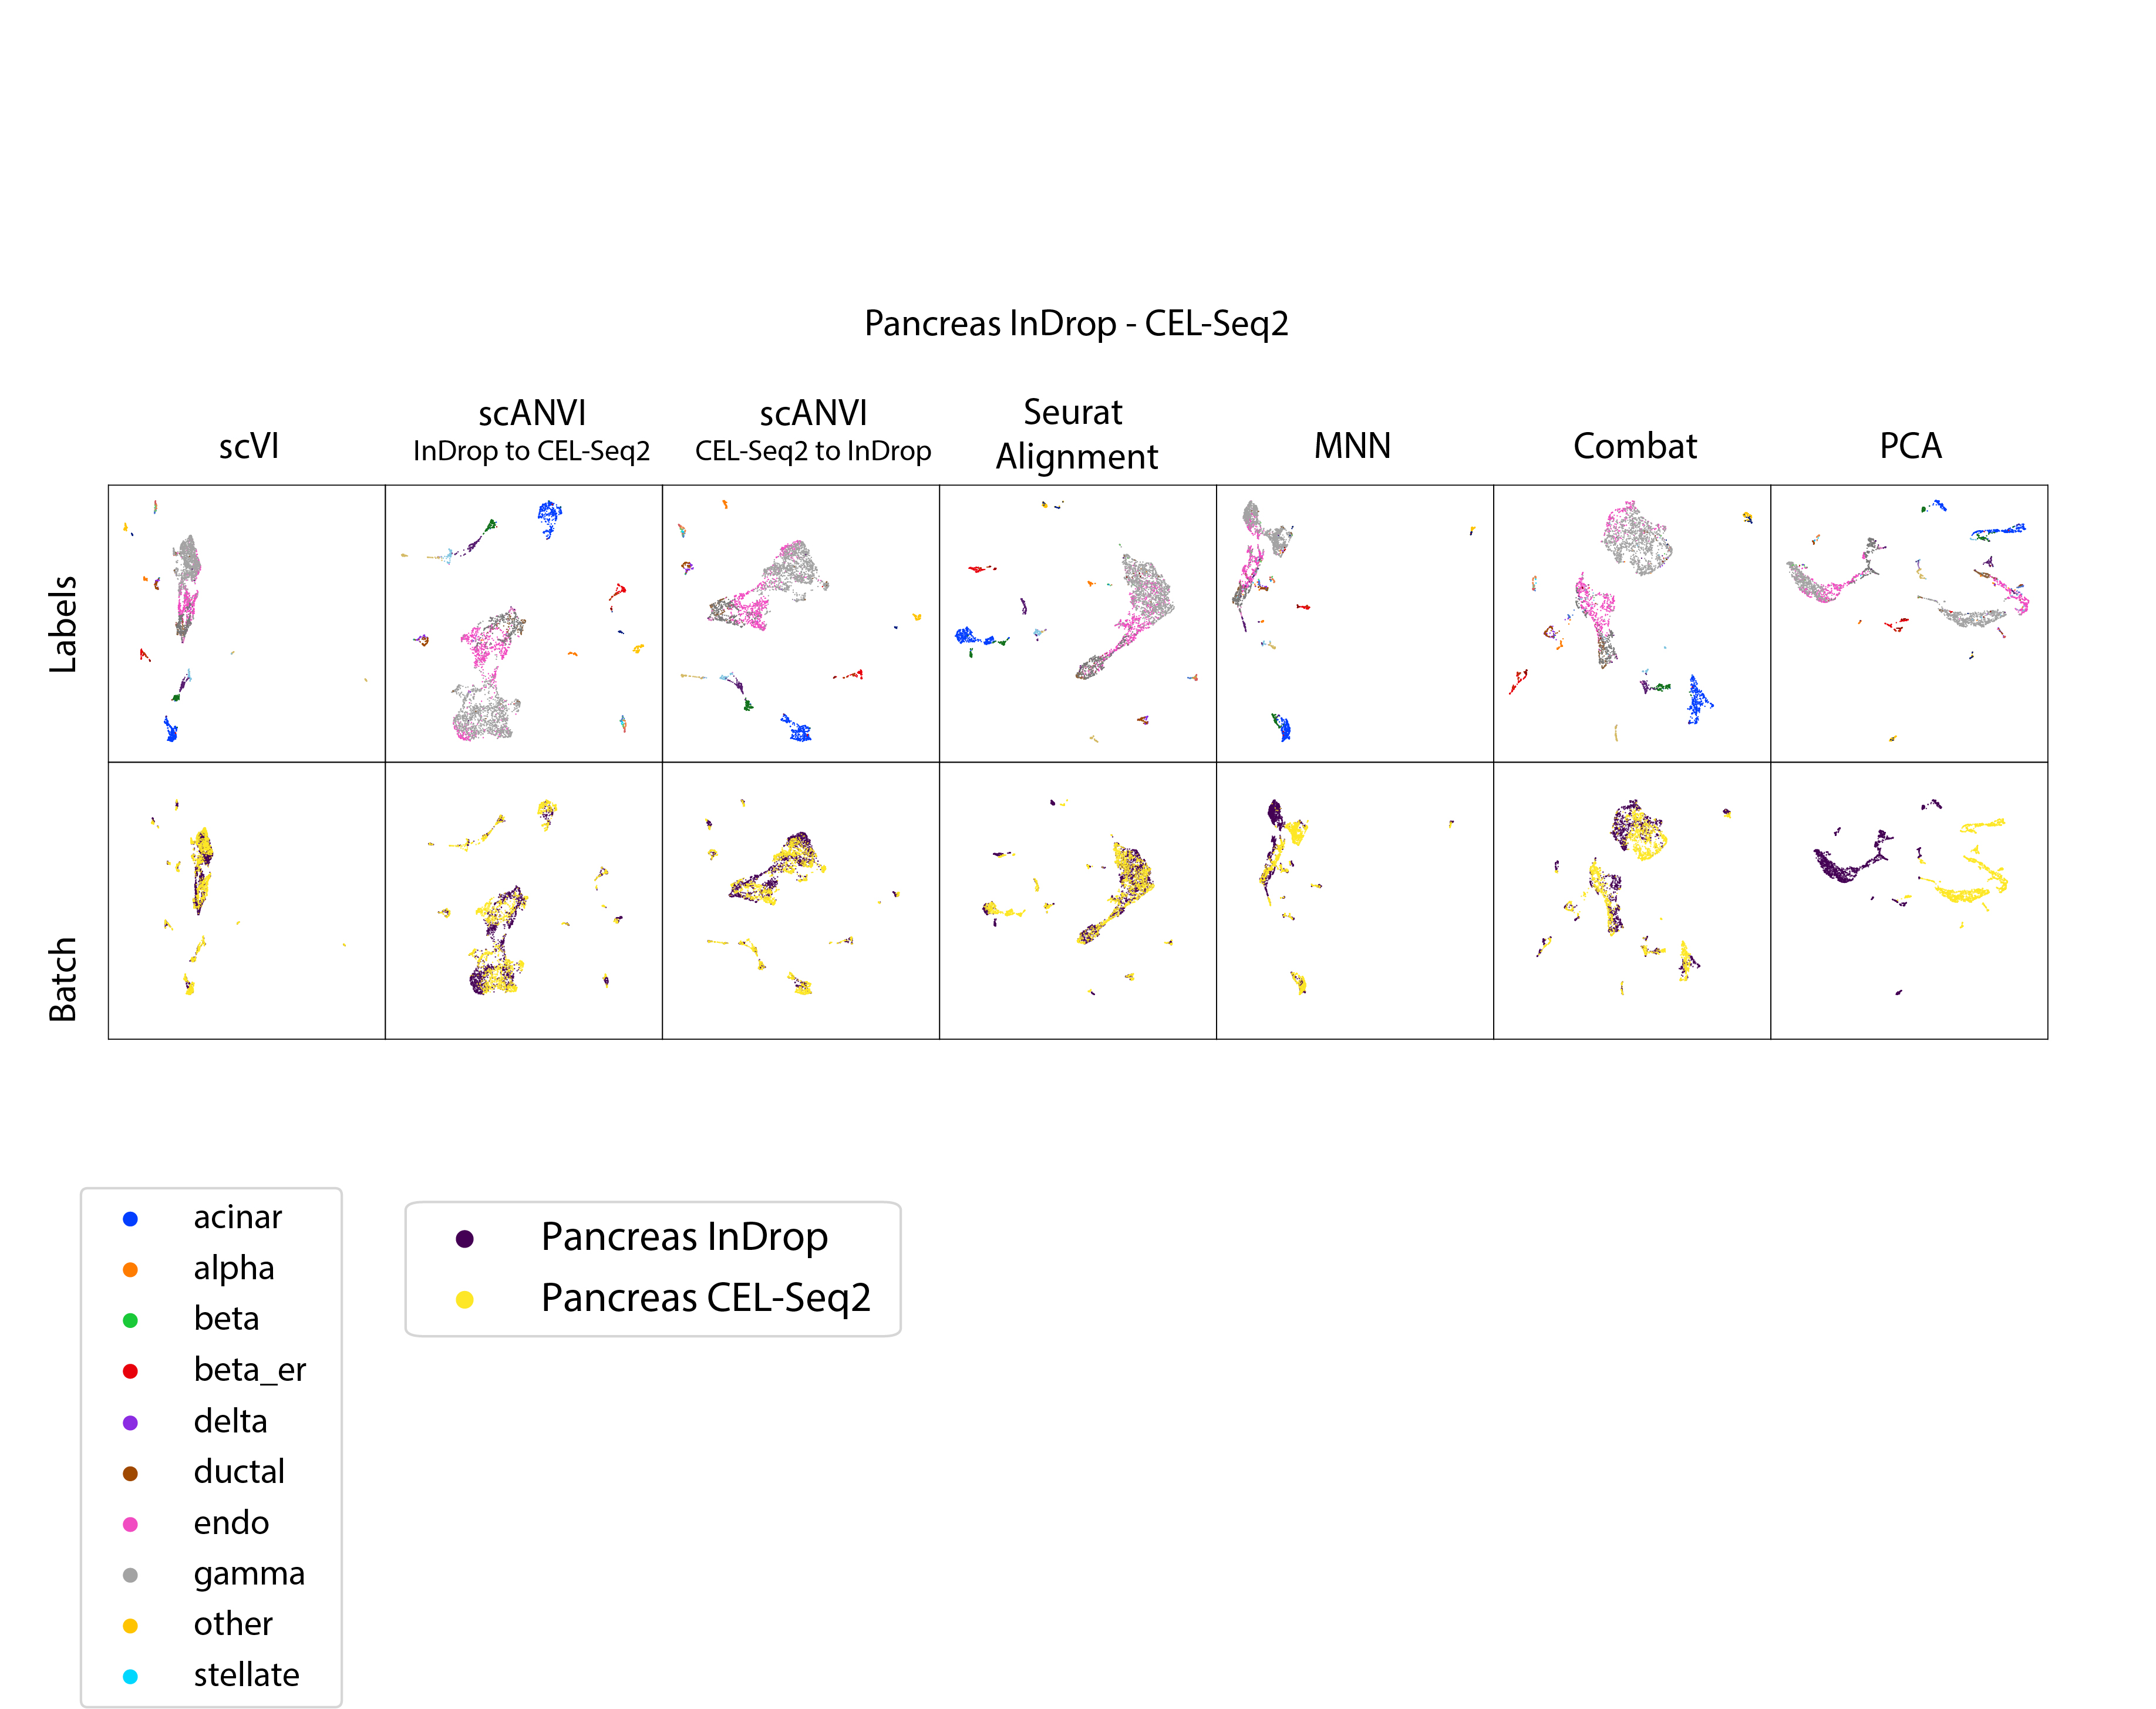
\includegraphics[width=\textwidth]{figures/supFig1-Tech3.jpg}
\caption[Visualization of the benchmark Pancreas InDrop / CEL-Seq2]{Visualization of the benchmark Pancreas InDrop / CEL-Seq2. All positions for the scatter plots are derived using UMAP on the latent space of interest.}
\label{scanviTech3}
\end{suppfigure}


\begin{suppfigure}[H]
\centering
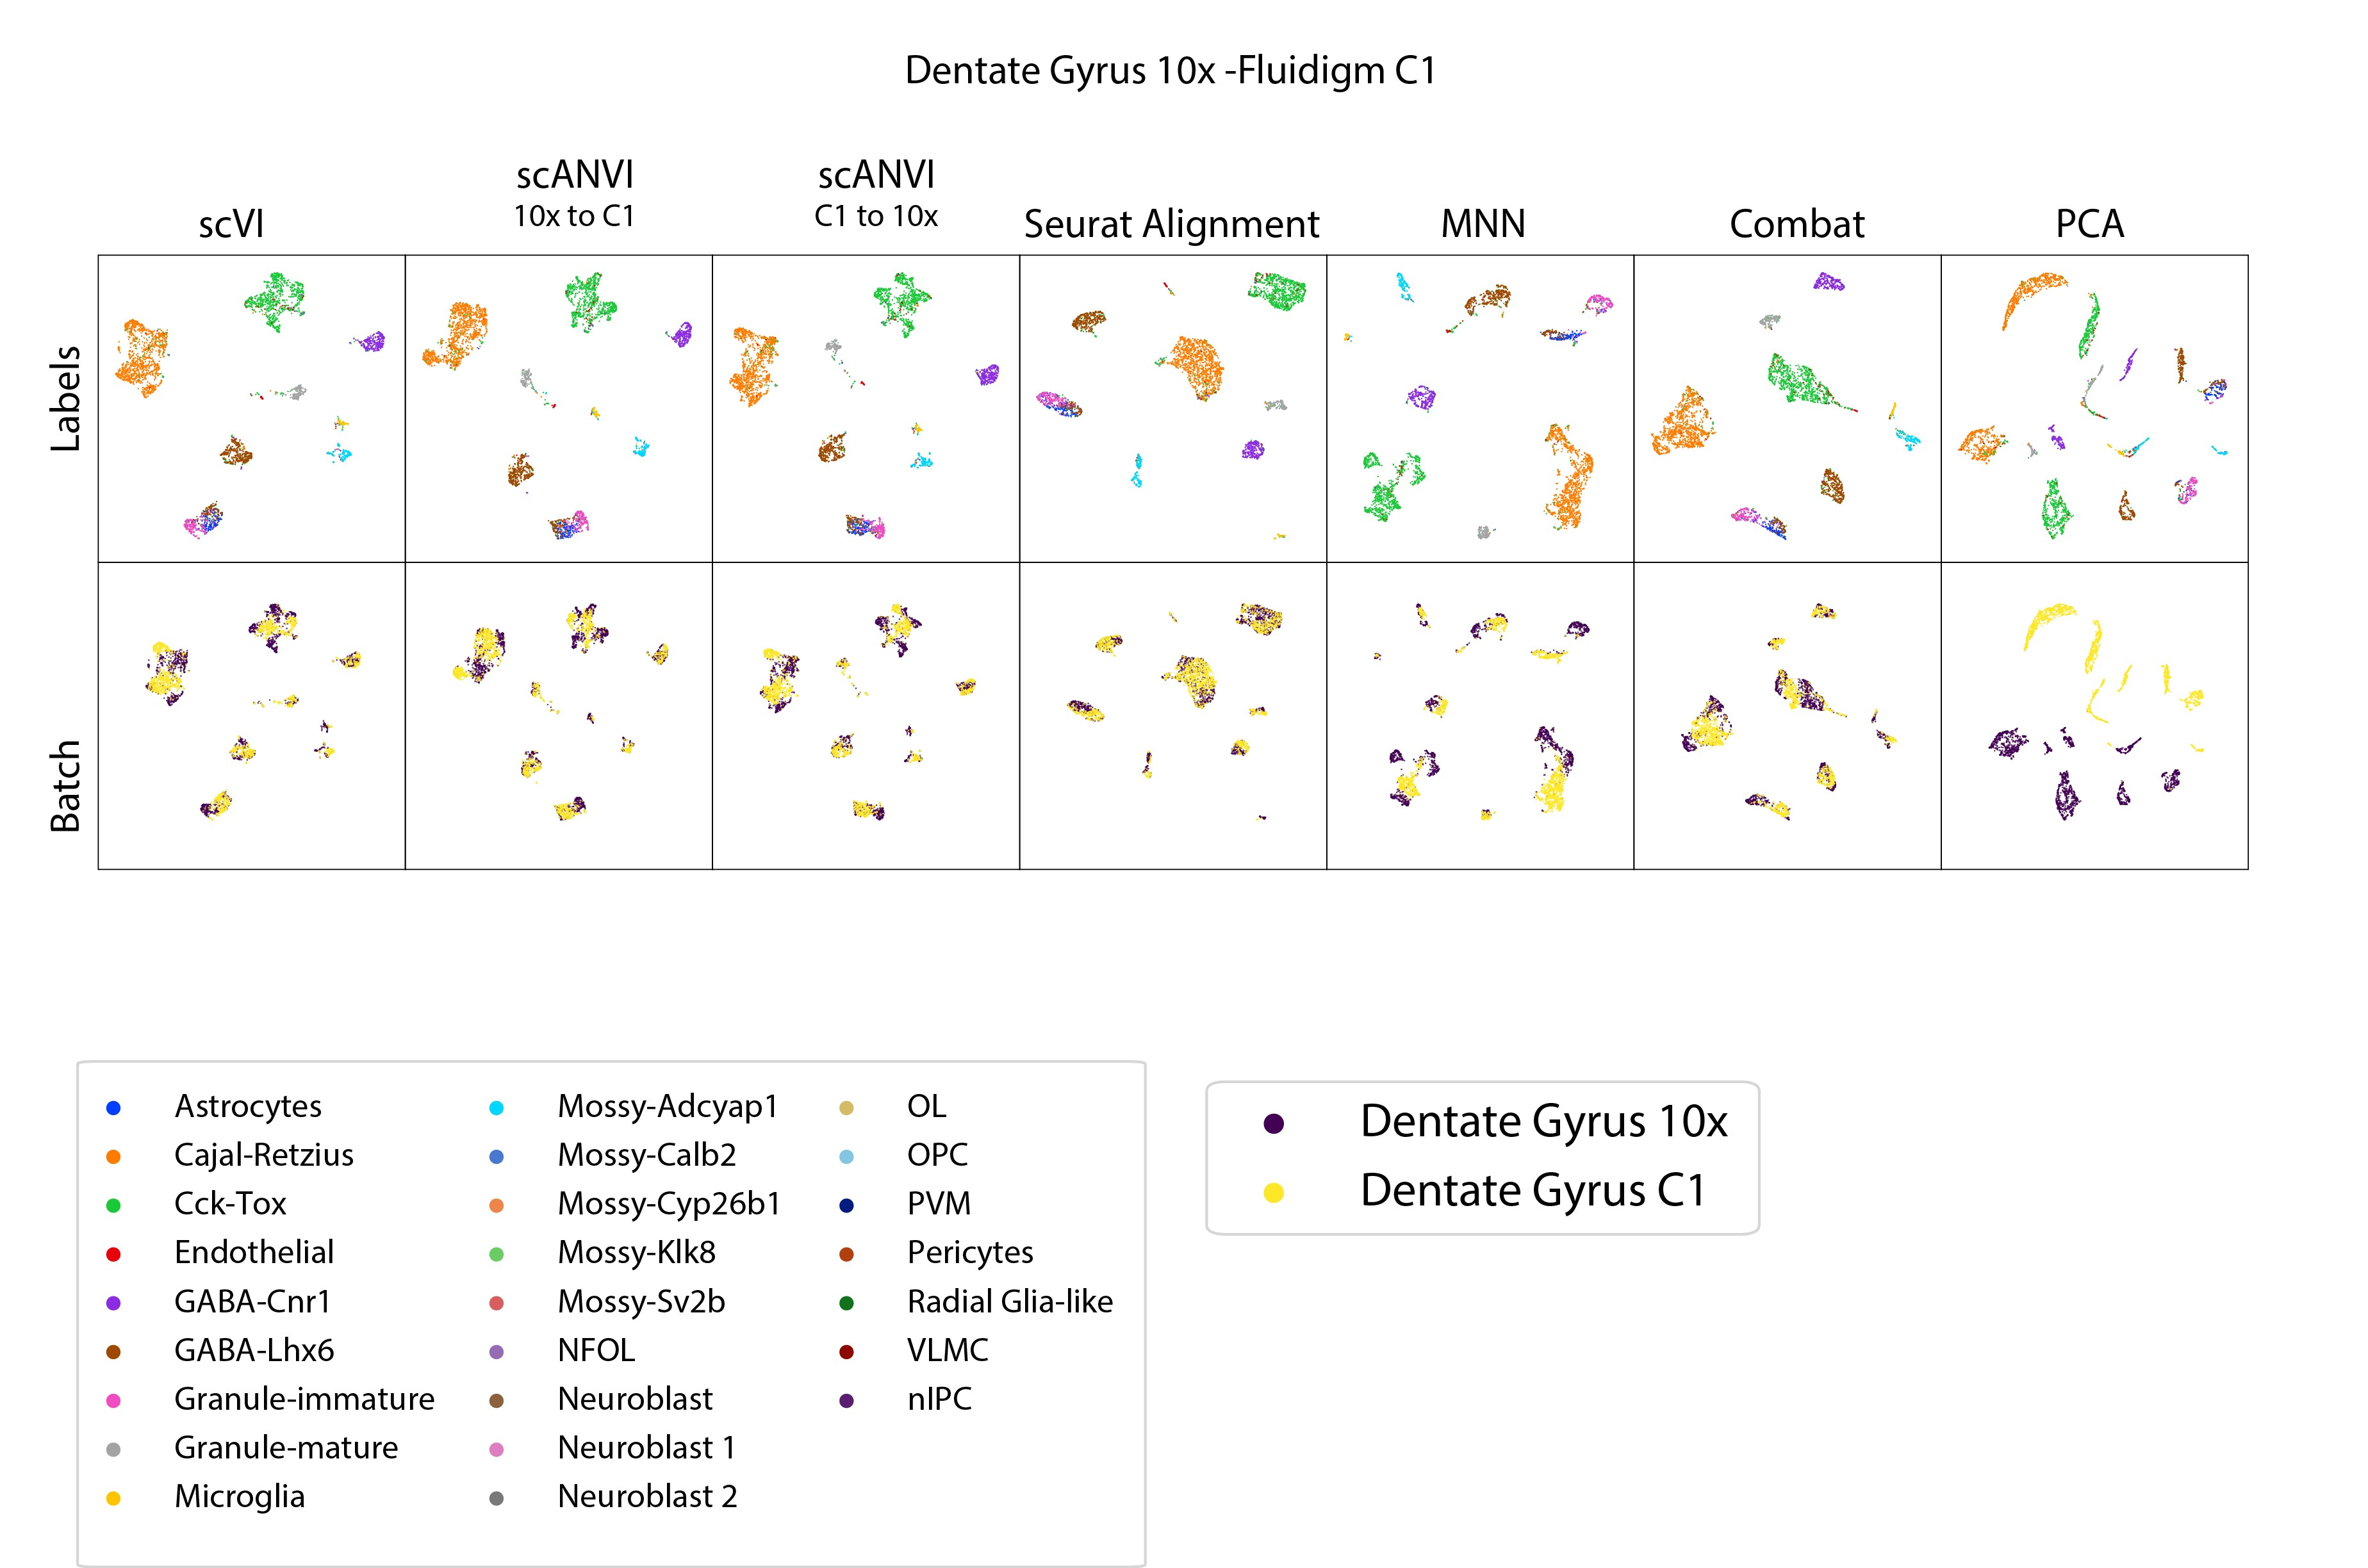
\includegraphics[width=\textwidth]{figures/supFig1-Tech4.jpg}
\caption[Visualization of the benchmark DentateGyrus10X - Fluidigm C1]{Visualization of the benchmark DentateGyrus10X - Fluidigm C1. All positions for the scatter plots are derived using UMAP on the latent space of interest.}
\label{scanviTech4}
\end{suppfigure}



\begin{suppfigure}[H]
    \centering
    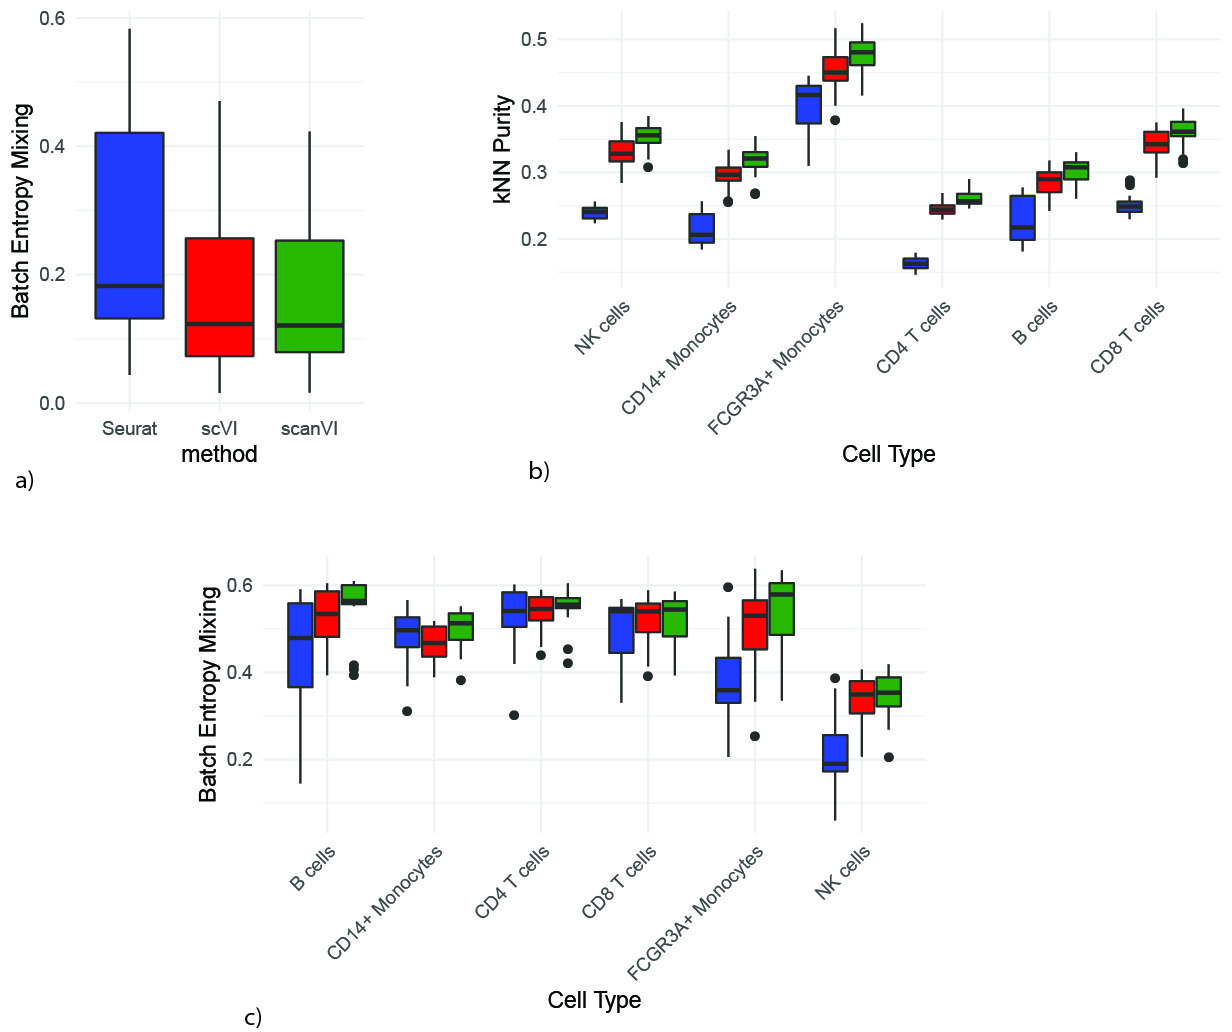
\includegraphics[width=\textwidth]{figures/unique_pops.jpg}
    \caption[Supplementary study of harmonizing datasets with different cellular composition]{Supplementary study of harmonizing datasets with different cellular composition. We show here the case where each of the two datasets has a unique cell types and share all the others. For each box plot, we report over all the possible combinations of left-out cell types. (a) Entropy of batch mixing for the unique population (lower is better). (b) $k$-nearest neighbor purity (unique and non-unique; higher is better). (c) Entropy of batch mixing for the non-unique populations (higher is better). The boxplots are standard Tukey boxplots where the box is delineated by the first and third quartile and the whisker lines are the first and third quartile plus minus 1.5 times the box height. The dots are outliers that fall above or below the whisker lines.}
    \label{scanviunique_pops}
\end{suppfigure}

\begin{suppfigure}[H]
\centering
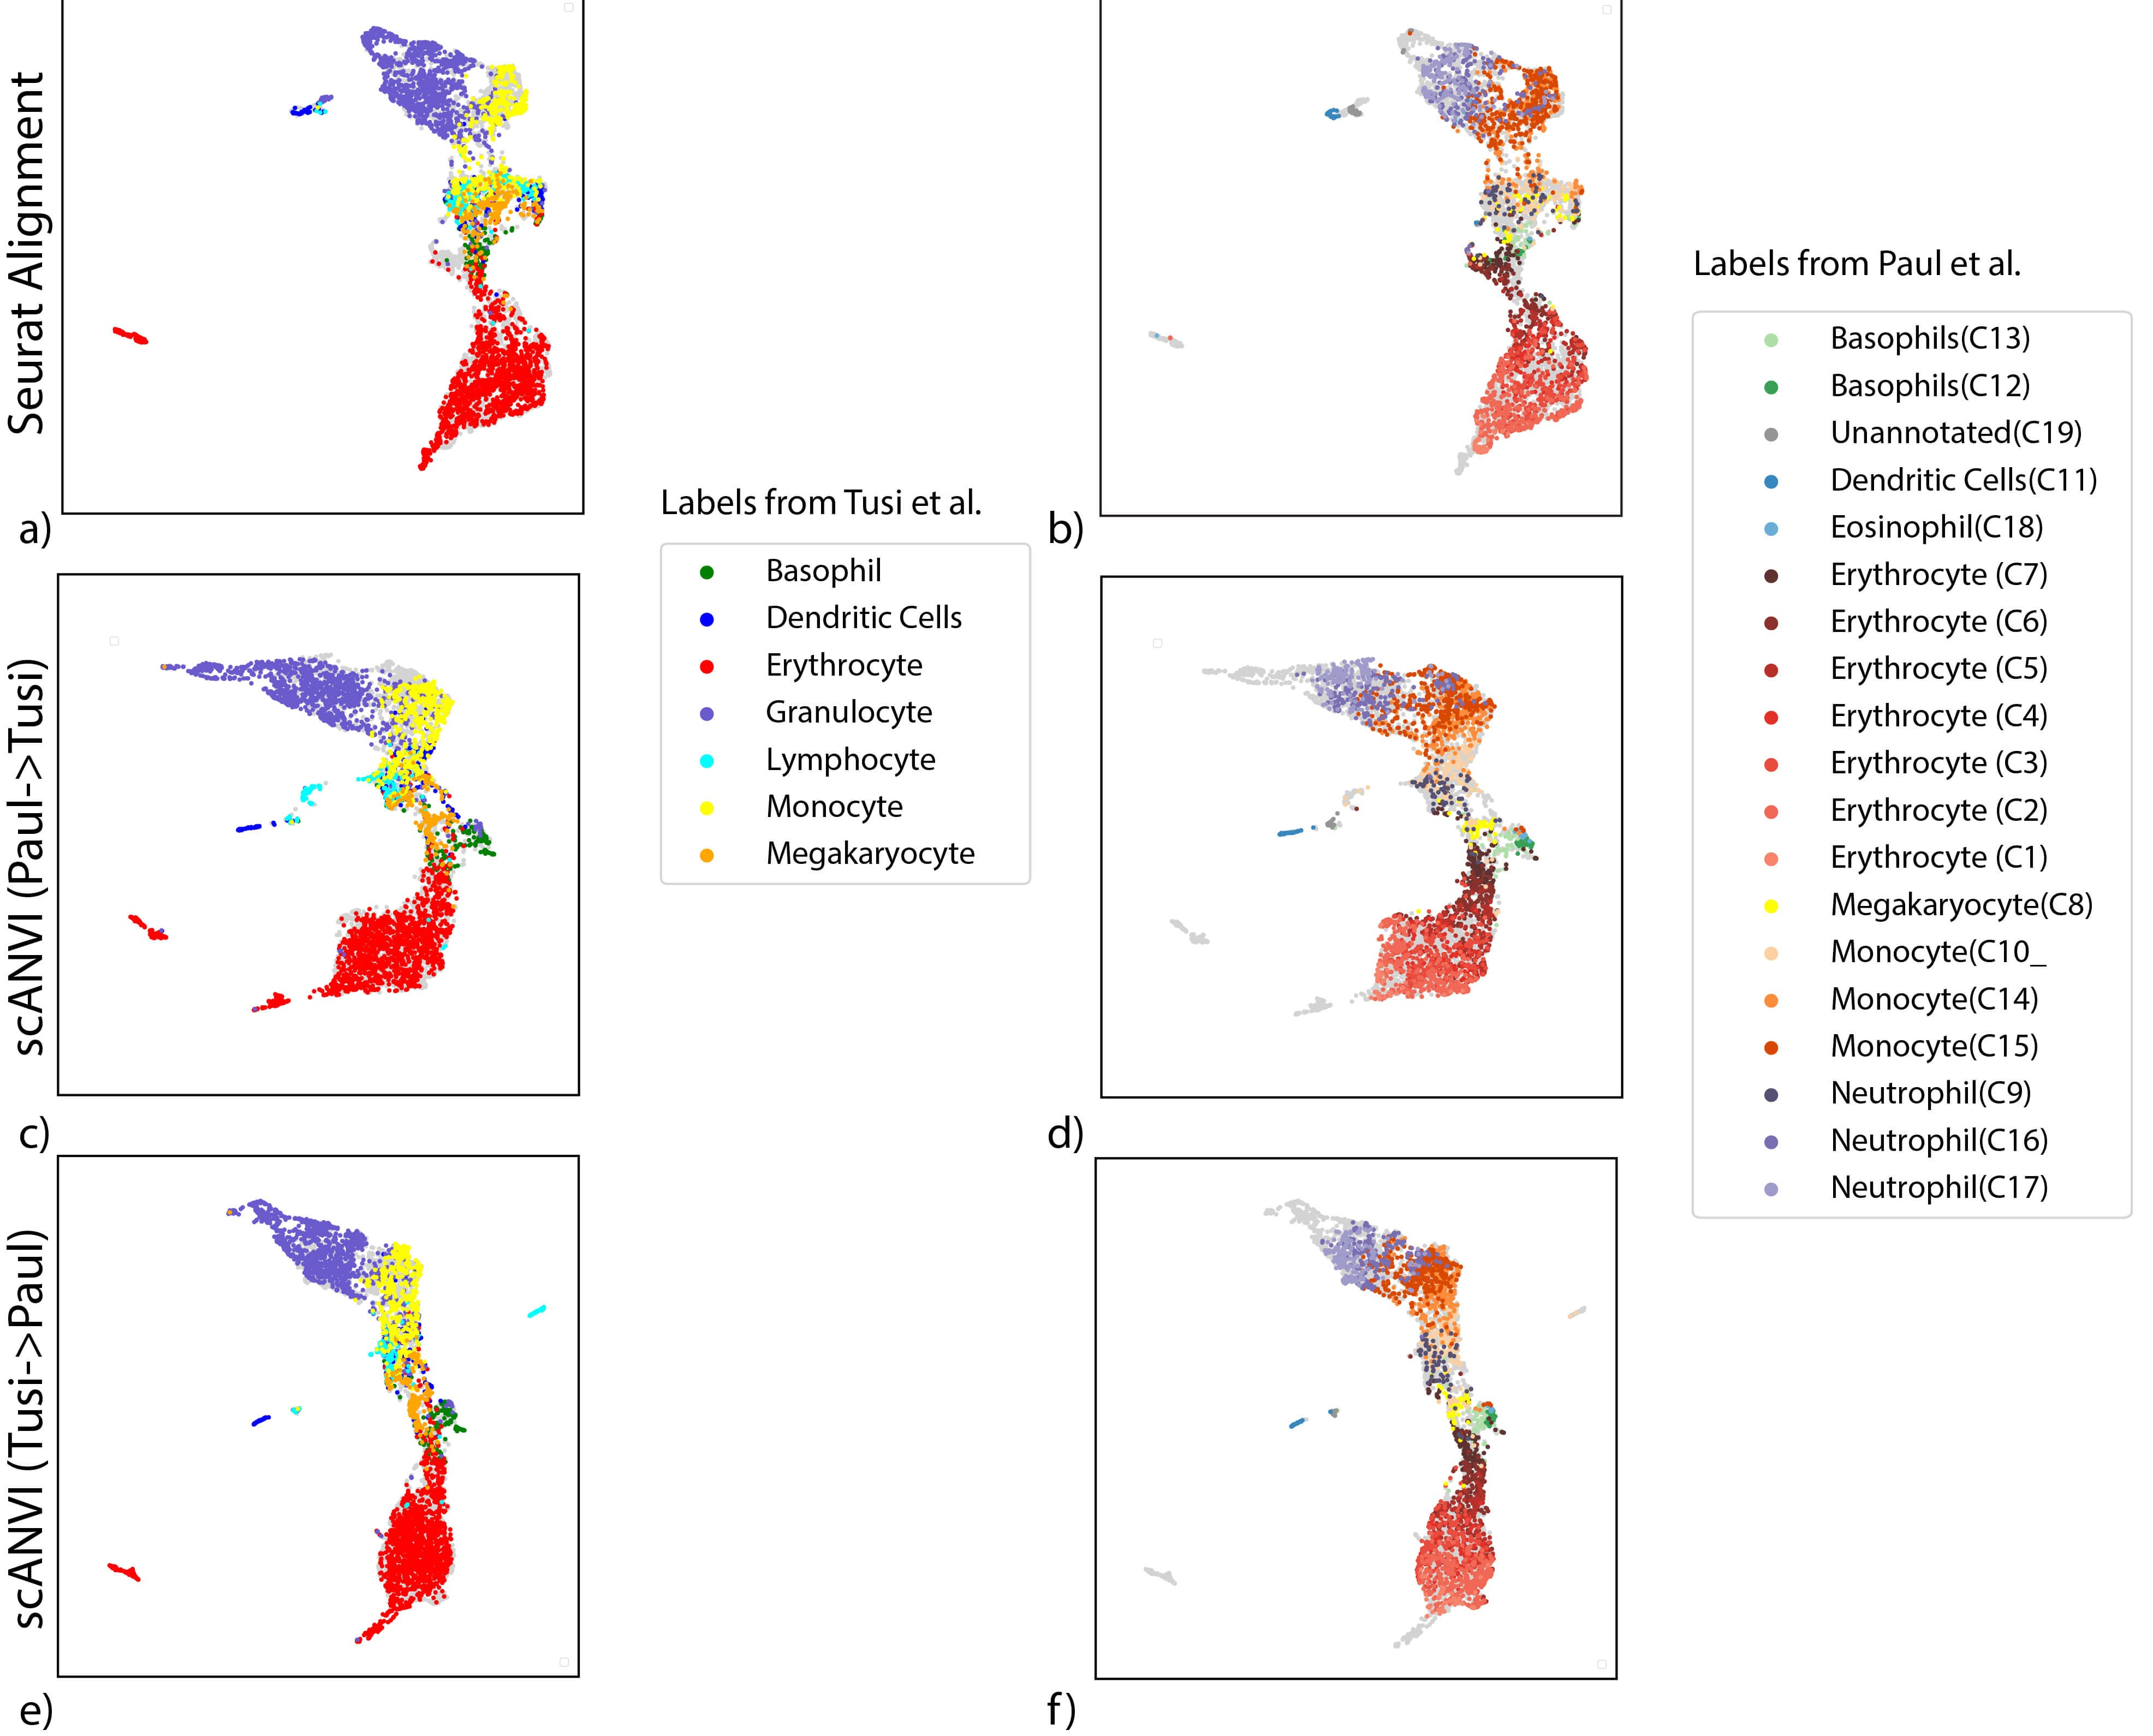
\includegraphics[width=\textwidth]{figures/continuous_supp.jpg}
\caption[Follow-up analysis on continuous trajectory harmonization with scANVI]{Follow-up analysis on continuous trajectory harmonization with scANVI. $(a-b)$ Continuous trajectory obtained by the Seurat Alignment procedure for the HEMATO-Tusi and the HEMATO-Paul datasets. $(c-d)$ Continuous trajectory obtained by the scANVI using the Tusi cell type labels for semi-supervision. $(e-f)$ Continuous trajectory obtained by the scANVI using the Paul cluster labels for semi-supervision.  All locations for scatter plots are computed via UMAP in their respective latent space. }
\label{scanvicontinuousSupp}
\end{suppfigure}


\begin{suppfigure}[H]
\centering
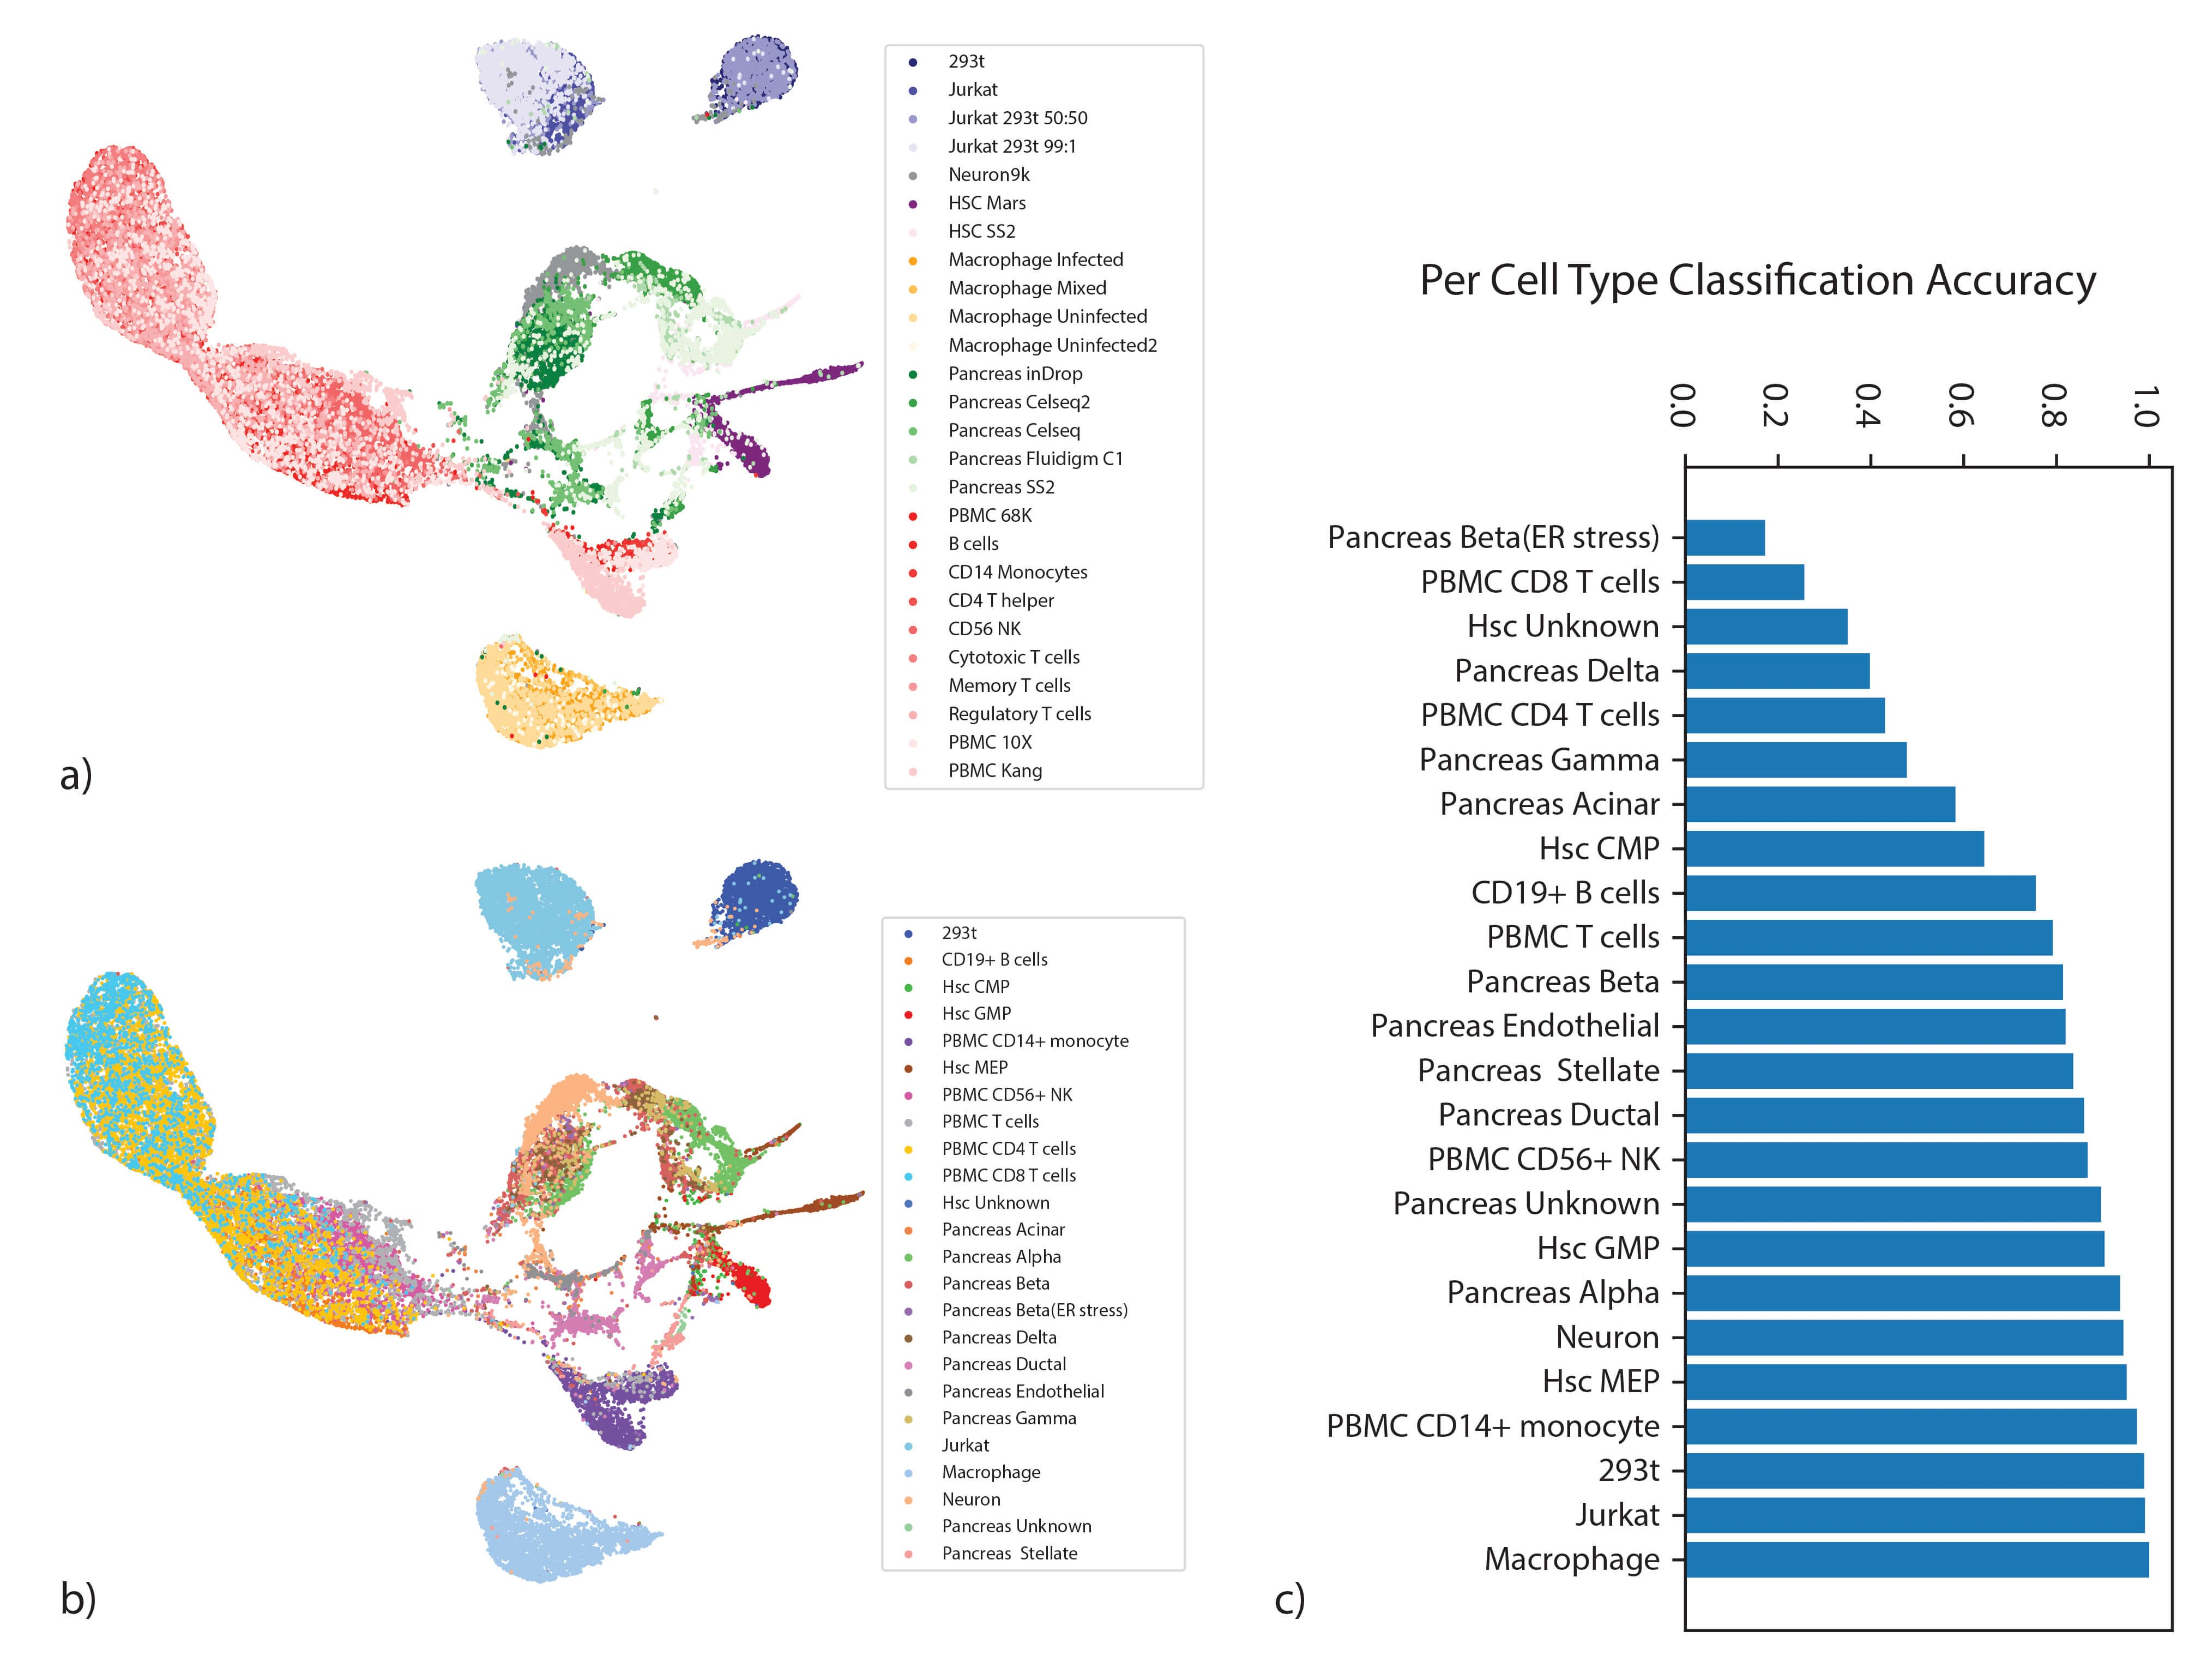
\includegraphics[width=\textwidth]{figures/scanorama.jpg}
\caption[Large-scale data integration with scVI]{Large-scale data integration with scVI. $(a-b)$ UMAP visualization of the scVI latent space colored by datasets $(a)$ and by cell types $(b)$. $(c)$ accuracy of a nearest neighbor classifier based on scVI latent space}
\label{scanvilarge_scale_panel}
\end{suppfigure}

\begin{suppfigure}[H]
\centering
\includegraphics[width=0.7\textwidth]{figures/acc_boxplot.jpg}
\caption[Annotation results for all four dataset pairs (boxplot)]{Annotation results for all four dataset pairs. PBMC-8K / PBMC-cite $(a-b)$, MarrowMT-10X / MarrowMT-SS2 $(c-d)$, Pancreas InDrop-CELSeq2 $(e-f)$ and Dentate Gyrus 10X / Fluidigm C1 $(g-h)$. Accuracies for transferring annotations from one dataset to another from a $k$-nearest neighbors classifier on Seurat Alignment, and scVI latent space, scANVI, SCMAP and CORAL classifier are shown.  The aggregated results across for cell types that are shared between the two datasets is shown in box plots.  }
\label{scanviaccbox}
\end{suppfigure}

\begin{suppfigure}[H]
\centering
\includegraphics[width=0.9\textwidth]{figures/bubbles.jpg}
\caption[Annotation results for all four dataset pairs (bubbleplot)]{Annotation results for all four dataset pairs. PBMC-8K / PBMC-cite $(a-b)$, MarrowMT-10X / MarrowMT-SS2 $(c-d)$, Pancreas InDrop-CELSeq2 $(e-f)$ and Dentate Gyrus 10X / Fluidigm C1 $(g-h)$.  Accuracies for transferring annotations from one dataset to another from a $k$-nearest neighbors classifier on Seurat Alignment, and scVI latent space, scANVI, SCMAP and CORAL classifier are shown.  The prediction accuracy  for each cell type that is shared between the two datasets is shown on the y-axis and the size of the dots are proportional to the proportion of a cell type in the total population. }
\label{scanvibubble}
\end{suppfigure}


\begin{suppfigure}[H]
\centering
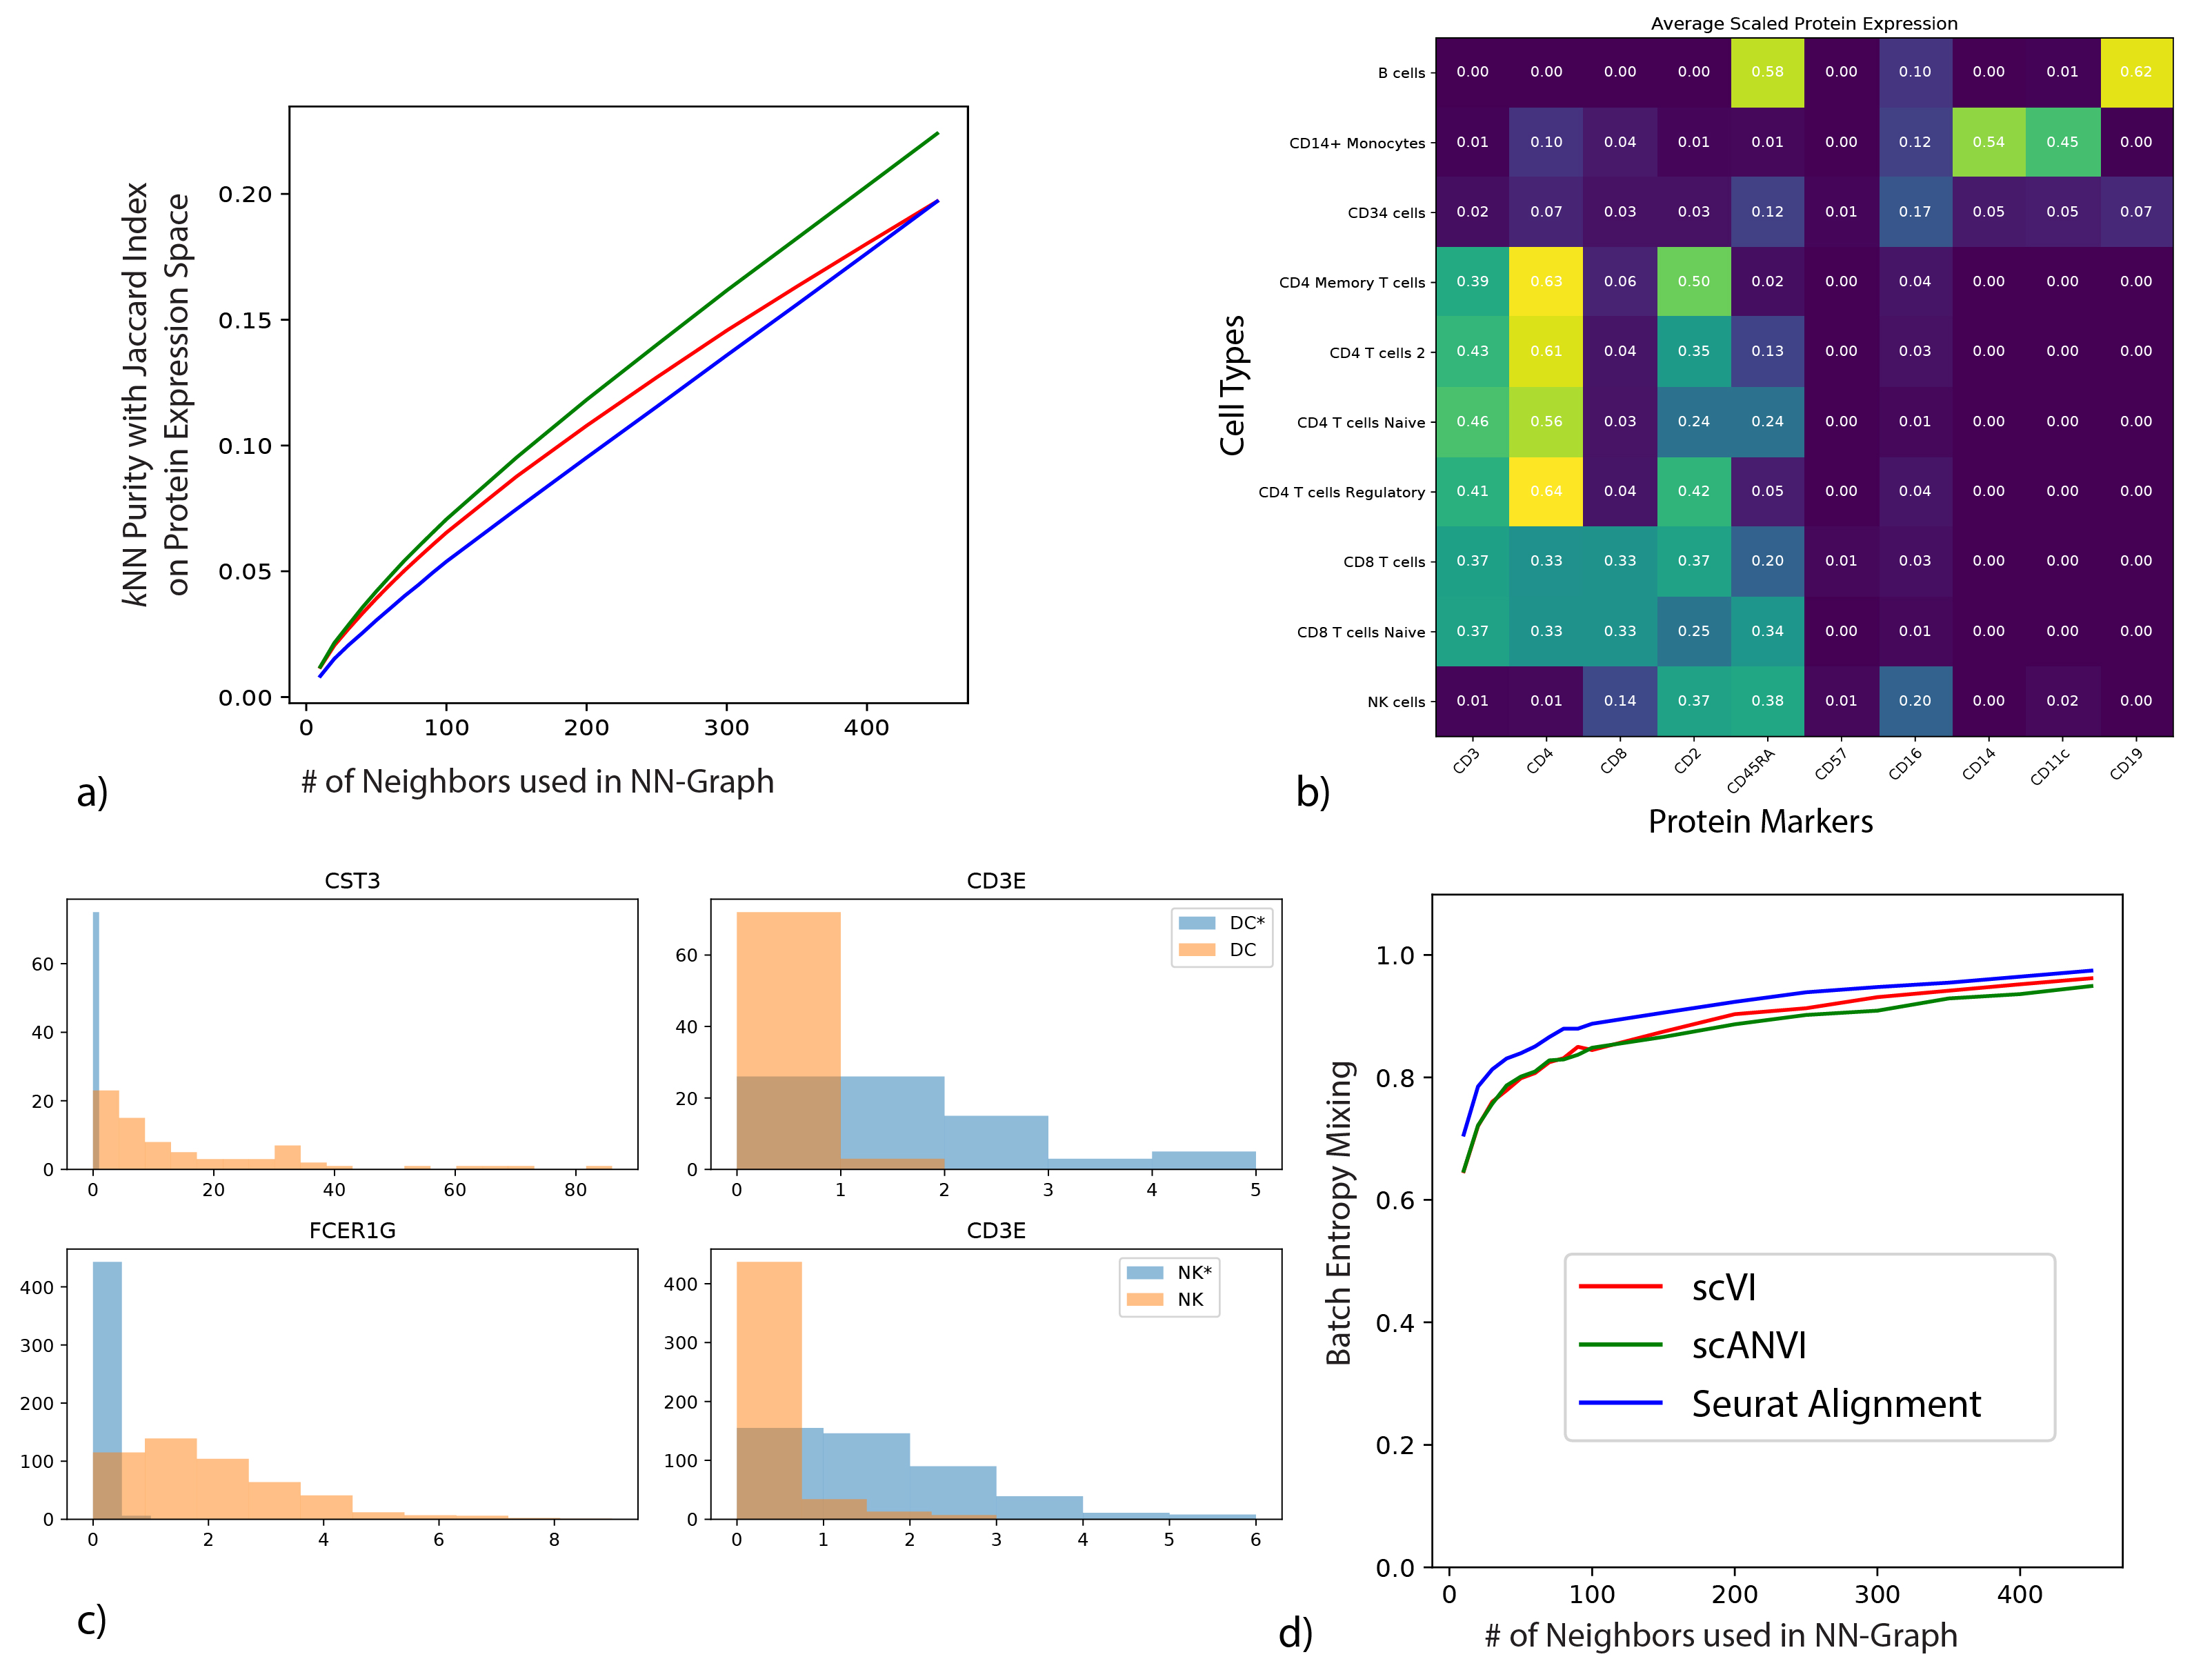
\includegraphics[width=\textwidth]{figures/labels_concored_supp.jpg}
\caption[Supplementary study of labels concordance]{Supplementary study of labels concordance. $(a)$ $k$-nearest neighbors purity of the merged latent space on the protein expression space as a function of the size of the neighborhood. $(b)$ Protein expression heatmap showing consistency of PBMC-Sorted labels and protein expression in PBMC-CITE. The protein expression per cell type is based on $k$-nearest neighbors imputation from the harmonized latent space obtained from scANVI trained with pure population labels. $(c)$ We select individual cells that were  labeled as dendritic cells or Natural Killer cells in the original publication of the respective datasets, and compare the raw transcript count from cells inside the scANVI T cells cluster (DC*, NK*) against cells outside the T cells cluster (DC, NK). The expression of marker genes suggest that DC* and NK* is more likely to be T cells and thus the scANVI latent space is more accurate. $(d)$ The batch entropy mixing of the three datasets in scVI, scANVI and Seurat Alignment merged space. }
\label{scanviconcord_supplement}
\end{suppfigure}




\begin{suppfigure}[H]
\centering
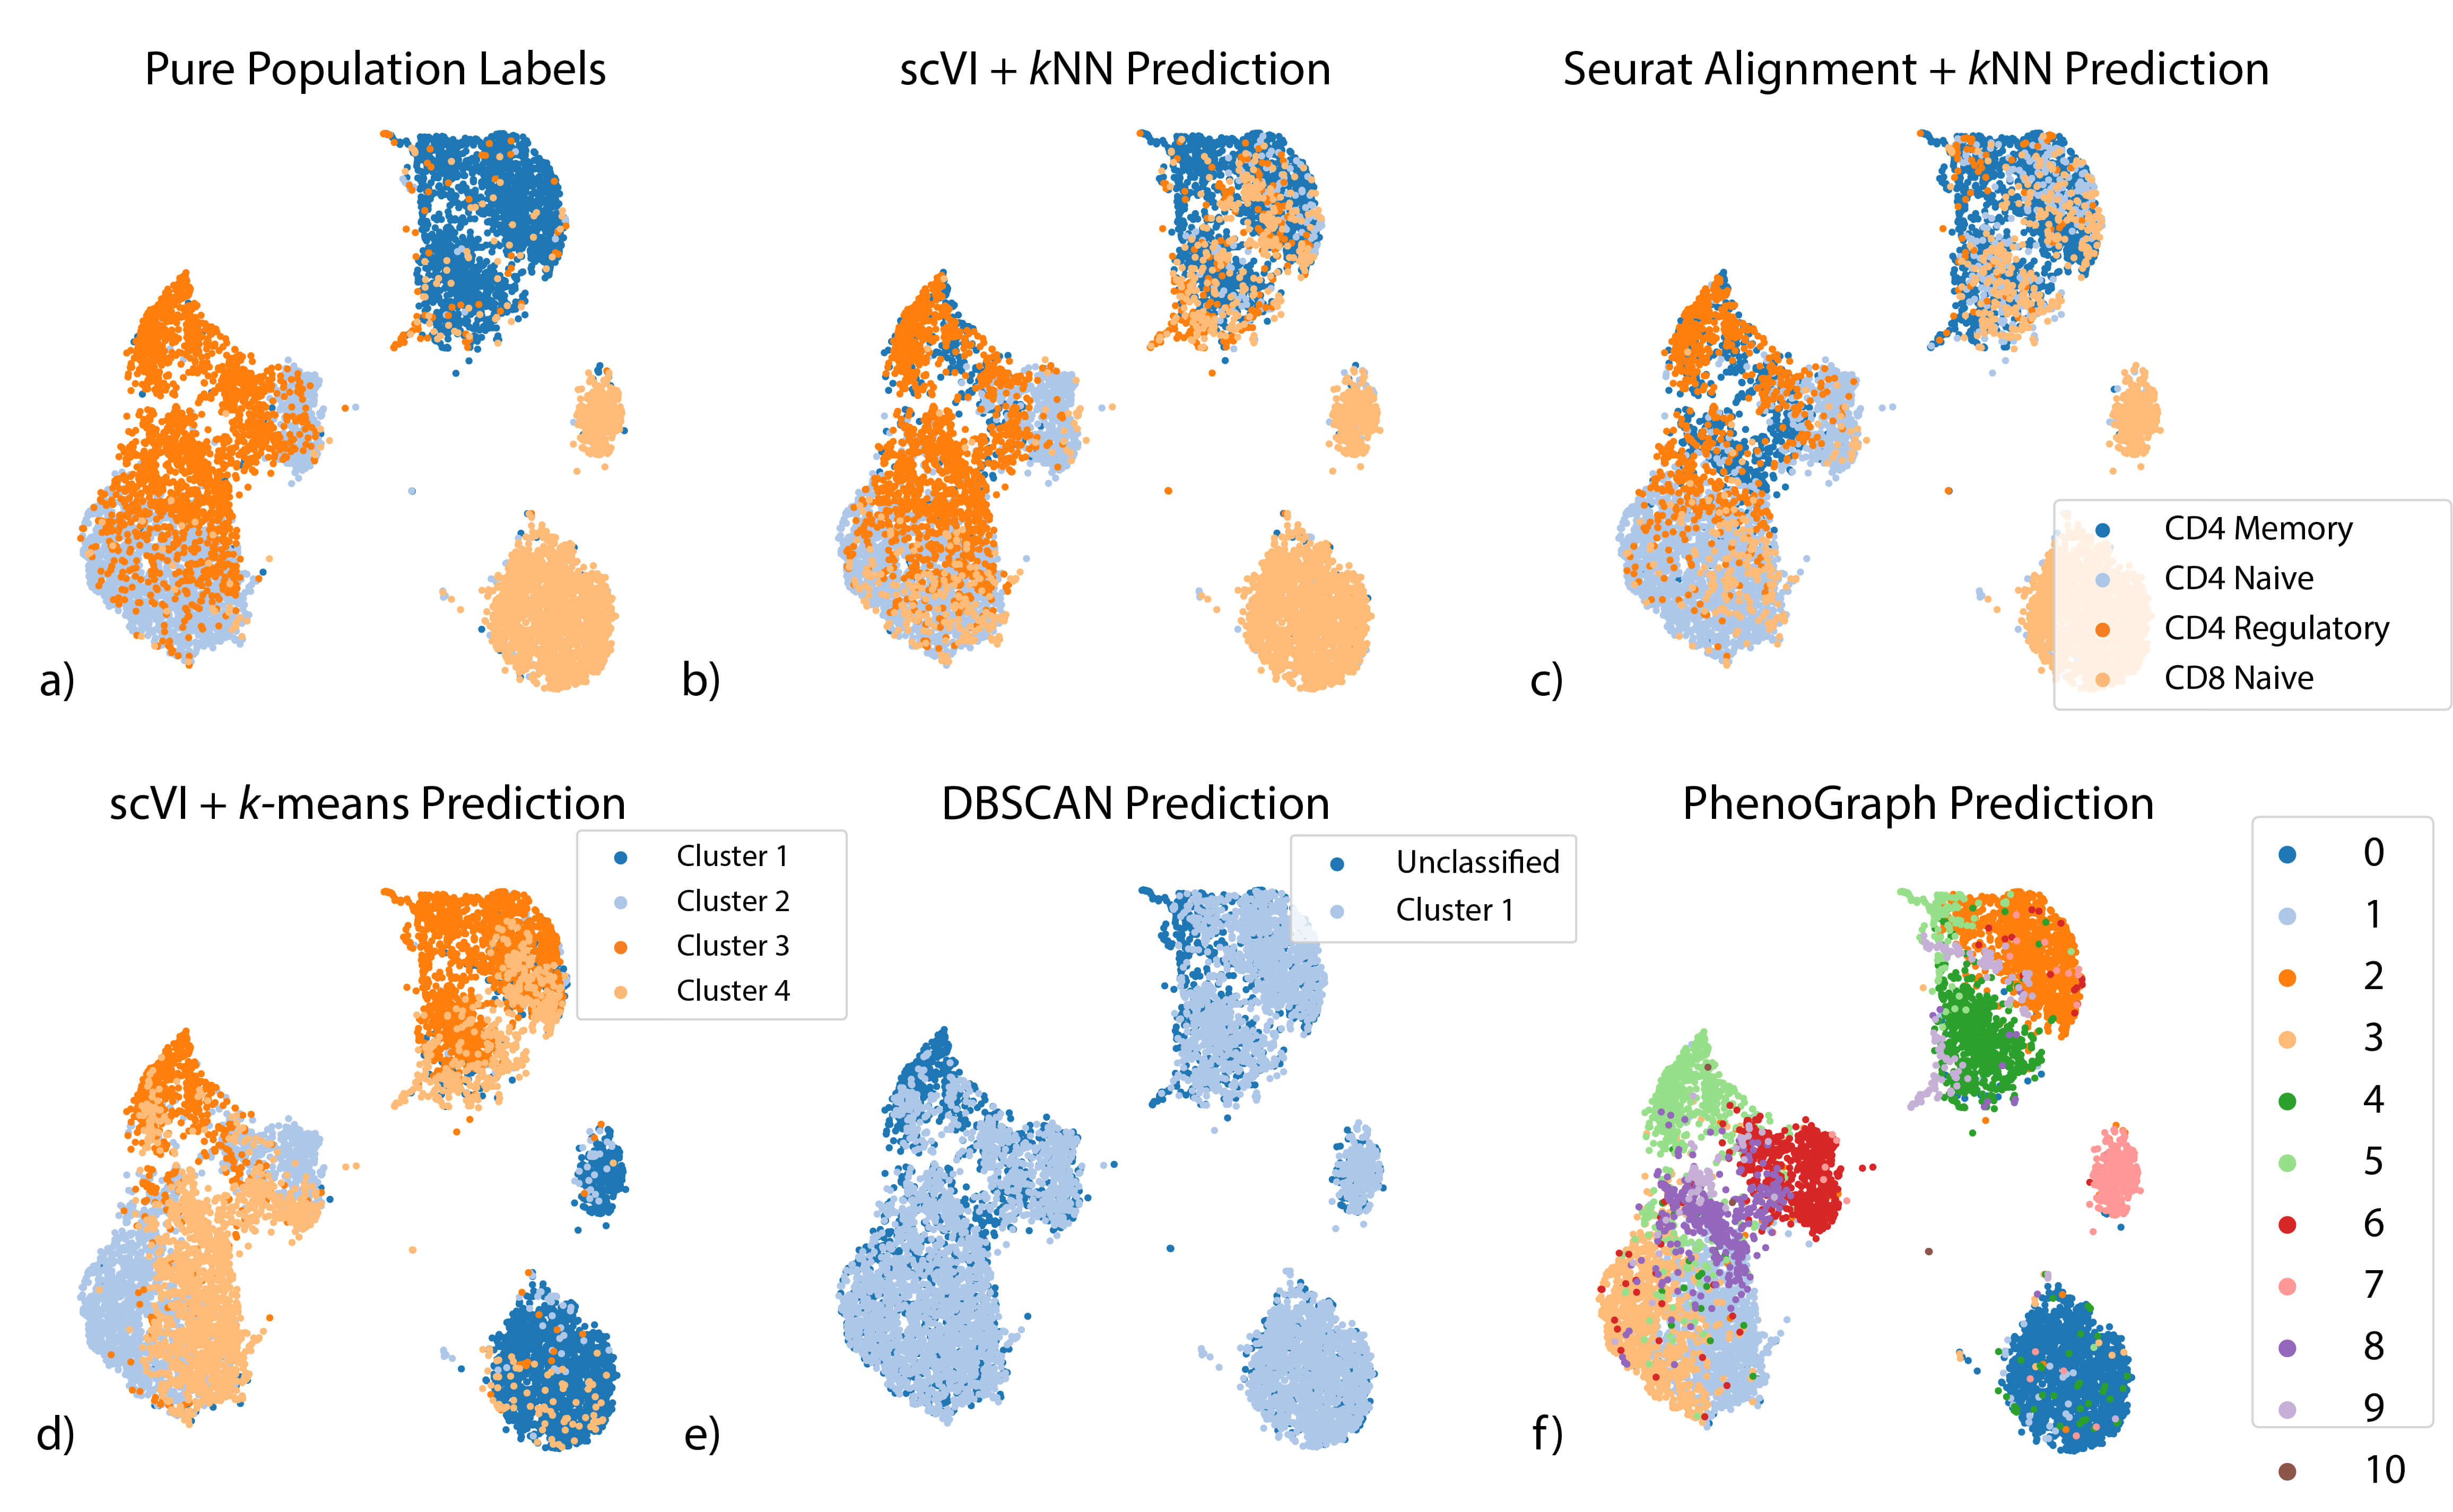
\includegraphics[width=\textwidth]{figures/scanvi_supp.jpg}
\caption[Other methods of classifying T-cell subsets of the PBMC-Pure dataset]{Other methods of classifying T-cell subsets of the PBMC-Pure dataset. Coordinates for the scatter plots are derived from UMAP embedding based on the latent space of scANVI. $(a)$ Ground truth labels from the purified PBMC populations $(b)$ $k$-nearest neighbors classification labels when applied on scVI latent space from the seed set of cells $(c)$ $k$-nearest neighbors classification labels when applied on Seurat Alignment latent space $(d)$ $k$-means clustering based labels when applied to scVI latent space $(e)$ DBSCAN clustering based labels when applied to scVI latent space. DBSCAN returns only one cluster but return some cells as unclassified. $(f)$ PhenoGraph clusters on scVI latent space}
\label{scanviscanviClustering}
\end{suppfigure}

\begin{suppfigure}[H]
    \centering
    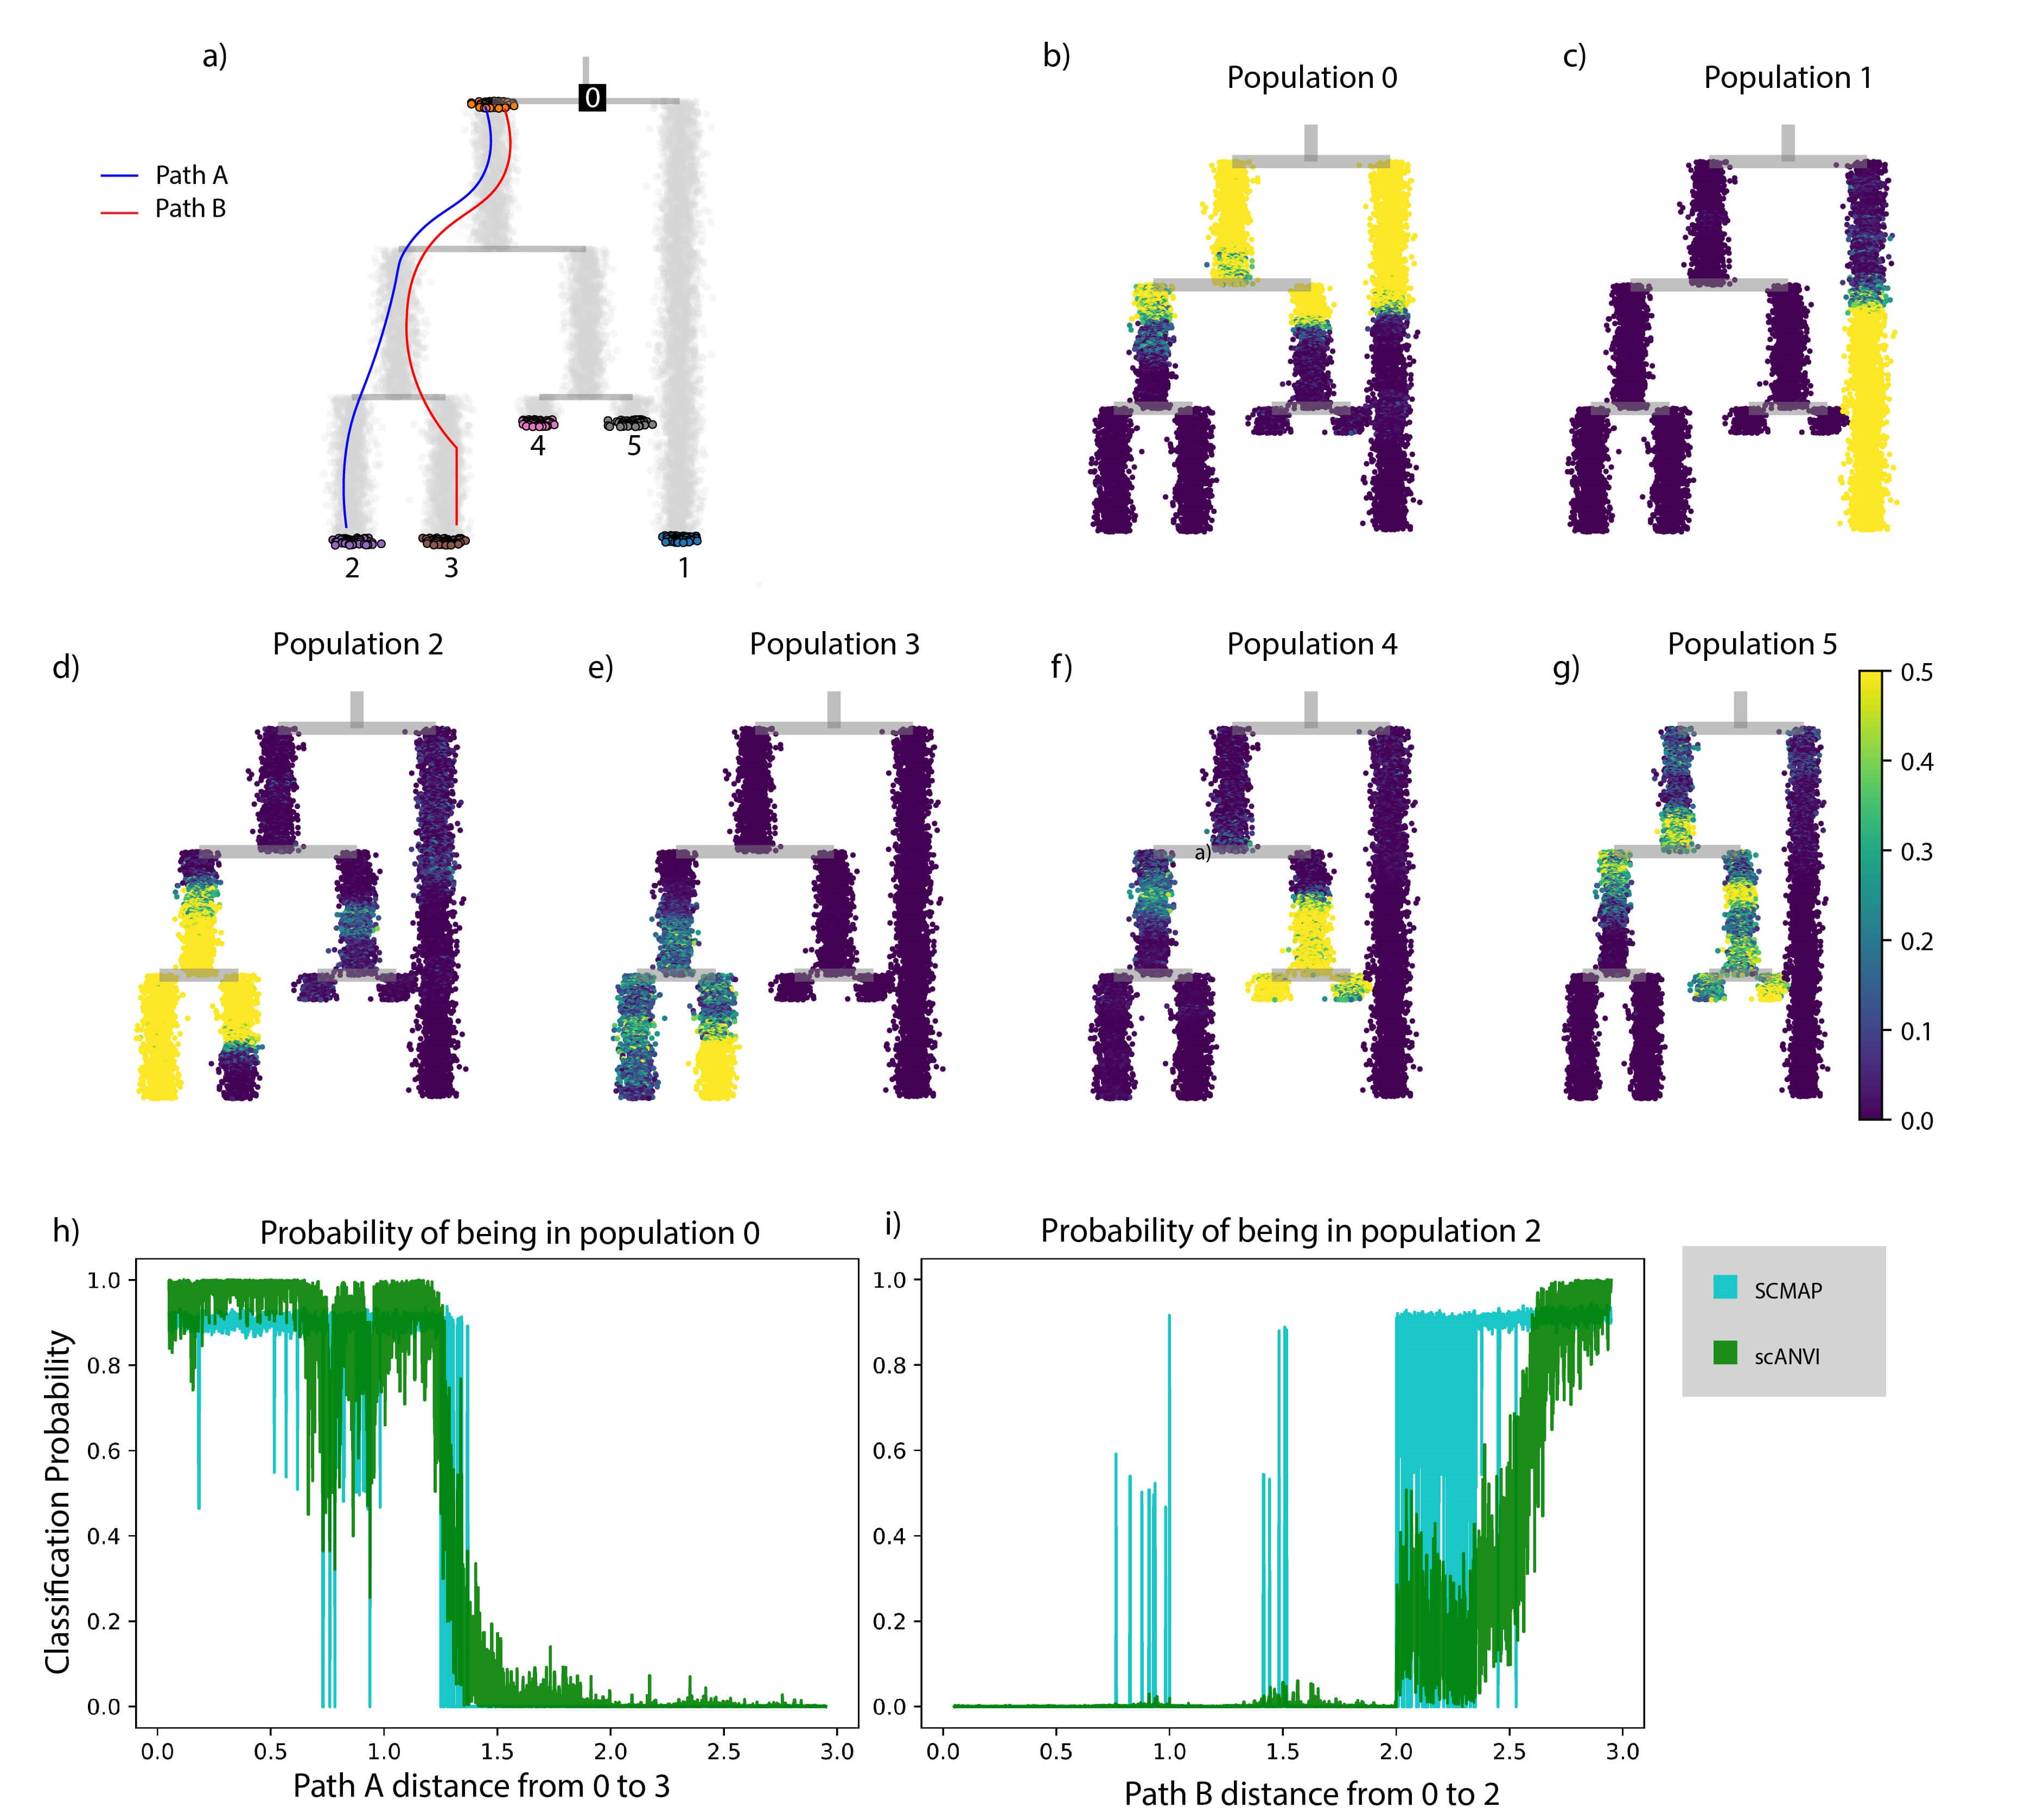
\includegraphics[width=\textwidth]{figures/symsim_continuous.jpg}
    \caption[Continuous trajectory simulated using SymSim]{Continuous trajectory simulated using SymSim. $(a)$ Tree structure from which the cells are sampled. Each grey dot represent a cell sampled along the trajectory. Colored dots with a black edge are treated as labeled, while the others are treated as unlabeled. Each path simulates a continuous phenotypical variation. $(b-g)$ The same tree with each cell colored by the posterior probability of being assigned to a specific label. $(h-i)$ Another visualization of the gradual change of posterior probability by plotting the posterior probability of root $(h)$ and population 3 $(i)$. The x-axis represents the pathwise distance (paths are defined in $(a)$), and the y-axis represents the probability, or confidence of the assignment.}
    \label{scanvisymsim_cont}
\end{suppfigure}

\begin{suppfigure}[H]
    \centering
    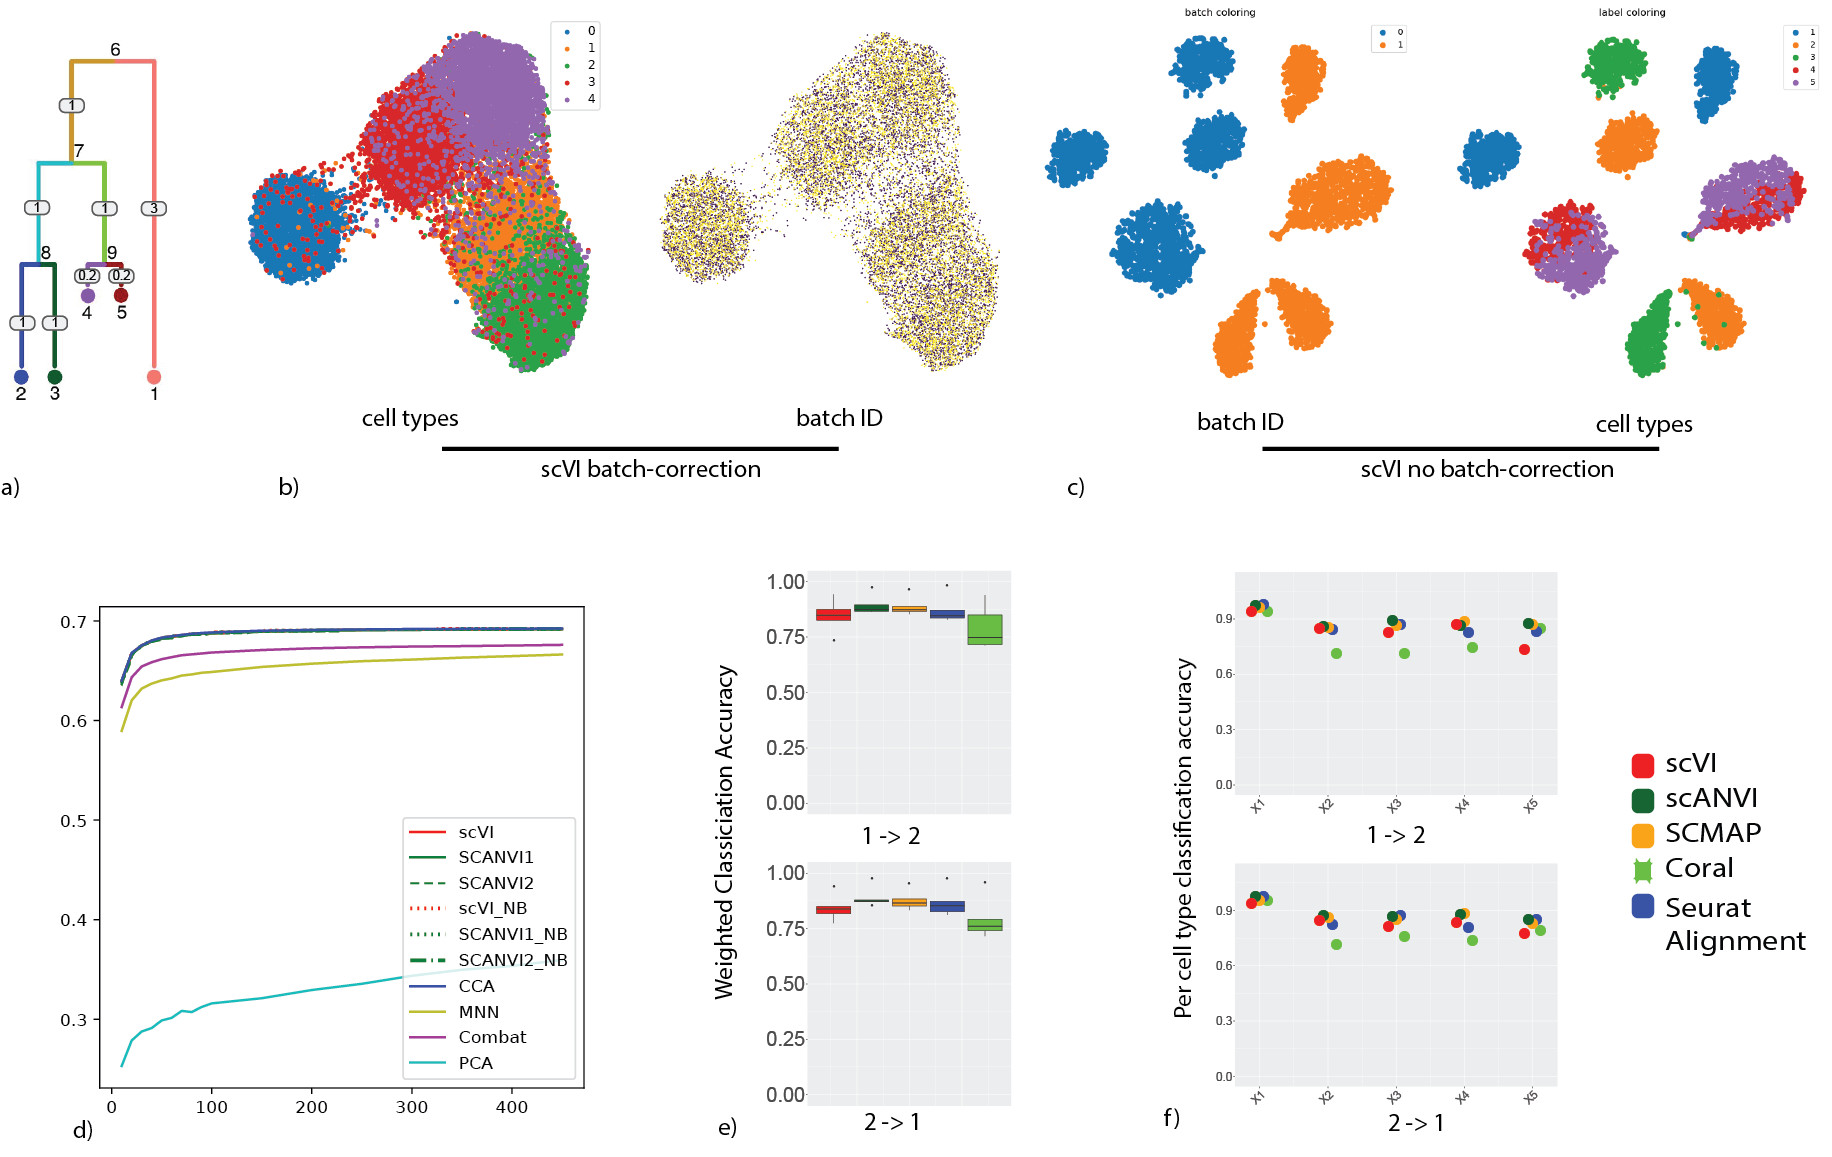
\includegraphics[width=\textwidth]{figures/panel_simulations.png}
    \caption[Presentation of the simulated dataset used for differential expression benchmarking]{Presentation of the simulated dataset used for differential expression benchmarking. (a) The tree used to sample the cells in SymSim. We sample cells from the five leaves nodes representing five different cell types derived from the same root node. (b) UMAP of scVI latent space colored by cell types and batch identifier (c) UMAP of scVI latent space without batch correction, proving that the data is indeed subject to batch effects. (d) Entropy of batch mixing for all the algorithms (e) Weighted accuracy using a $k$-nearest neighbors classifier on the latent space (f) Per cell type accuracy for the label transfer. }
    \label{scanvisimulations_panel}
\end{suppfigure}

\begin{suppfigure}[H]
\centering
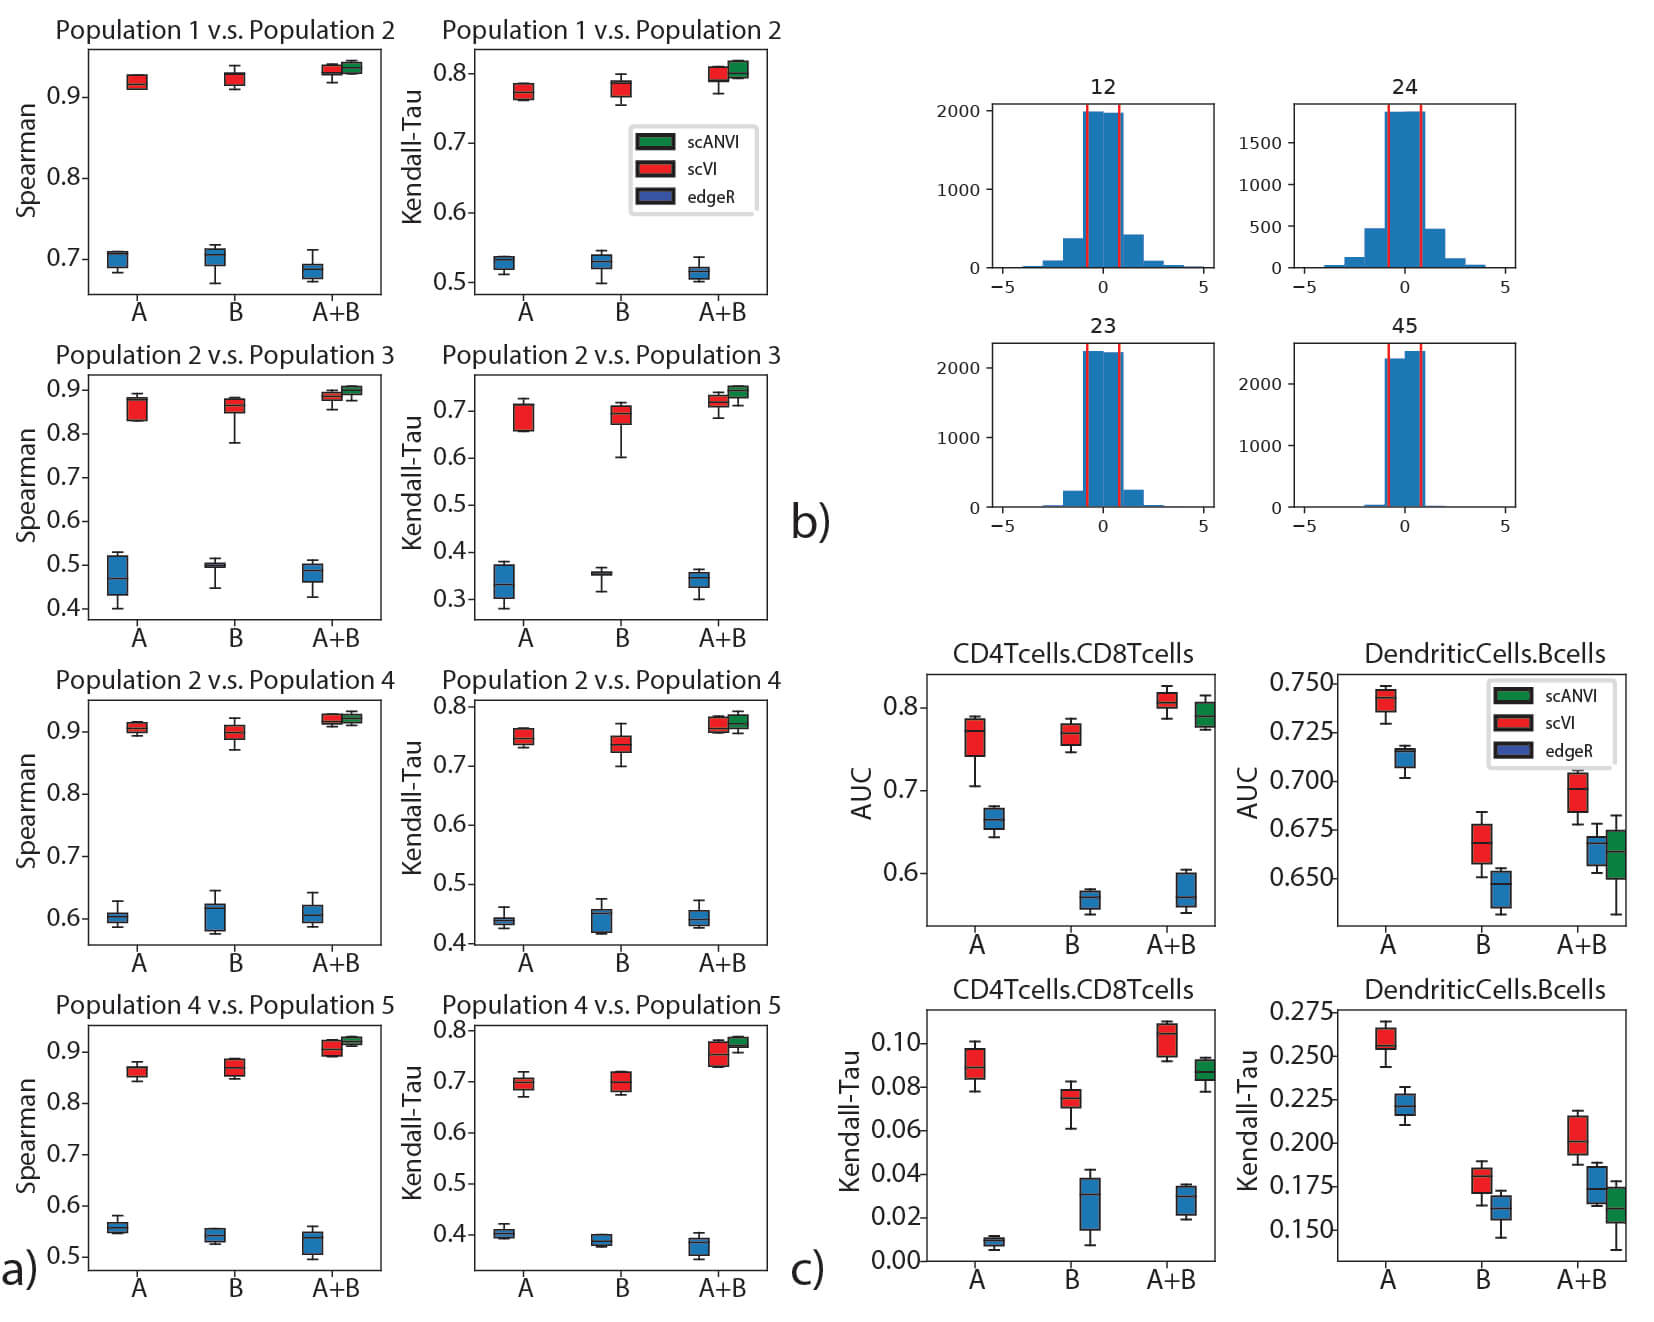
\includegraphics[width=\textwidth]{figures/de_new.jpg}
\caption[Differential Expression on multiple datasets with scVI]{Differential Expression on multiple datasets with scVI. $(a)$ Evaluation of consistency with rank correlation is shown for comparisons of multiple pairs of cell types in the simulated data. The pairs of cells are chosen to represent different levels of distance on the tree as in Figure~\ref{scanvisimulations_panel}a. The pairs of population from most distant to least distant are `12', `24', `23', `45'. $(b)$ distribution of true log fold change between all pairs of cell types for the simulated data. $(c)$ Evaluation of
consistency with the AUROC and Kendal Tau metric is shown for comparisons of CD4 vs CD8 T cells and B cells vs dendritic cells on the PBMC-8K only (A), the PBMC-68k only (B) and the merged PBMC-8K / PBMC-68K (A+B) for scVI and edgeR. Error bars are obtained by multiple subsampling
of the data to show robustness. Boxplots are standard Tukey boxplots where the box is delineated by the first and third quartile and the whisker lines are the first and third quartile plus minus 1.5 times the box height. The dots are outliers that fall above or below the whisker lines.}
\label{scanviDE_panel}
\end{suppfigure}

\begin{suppfigure}[H]
\centering
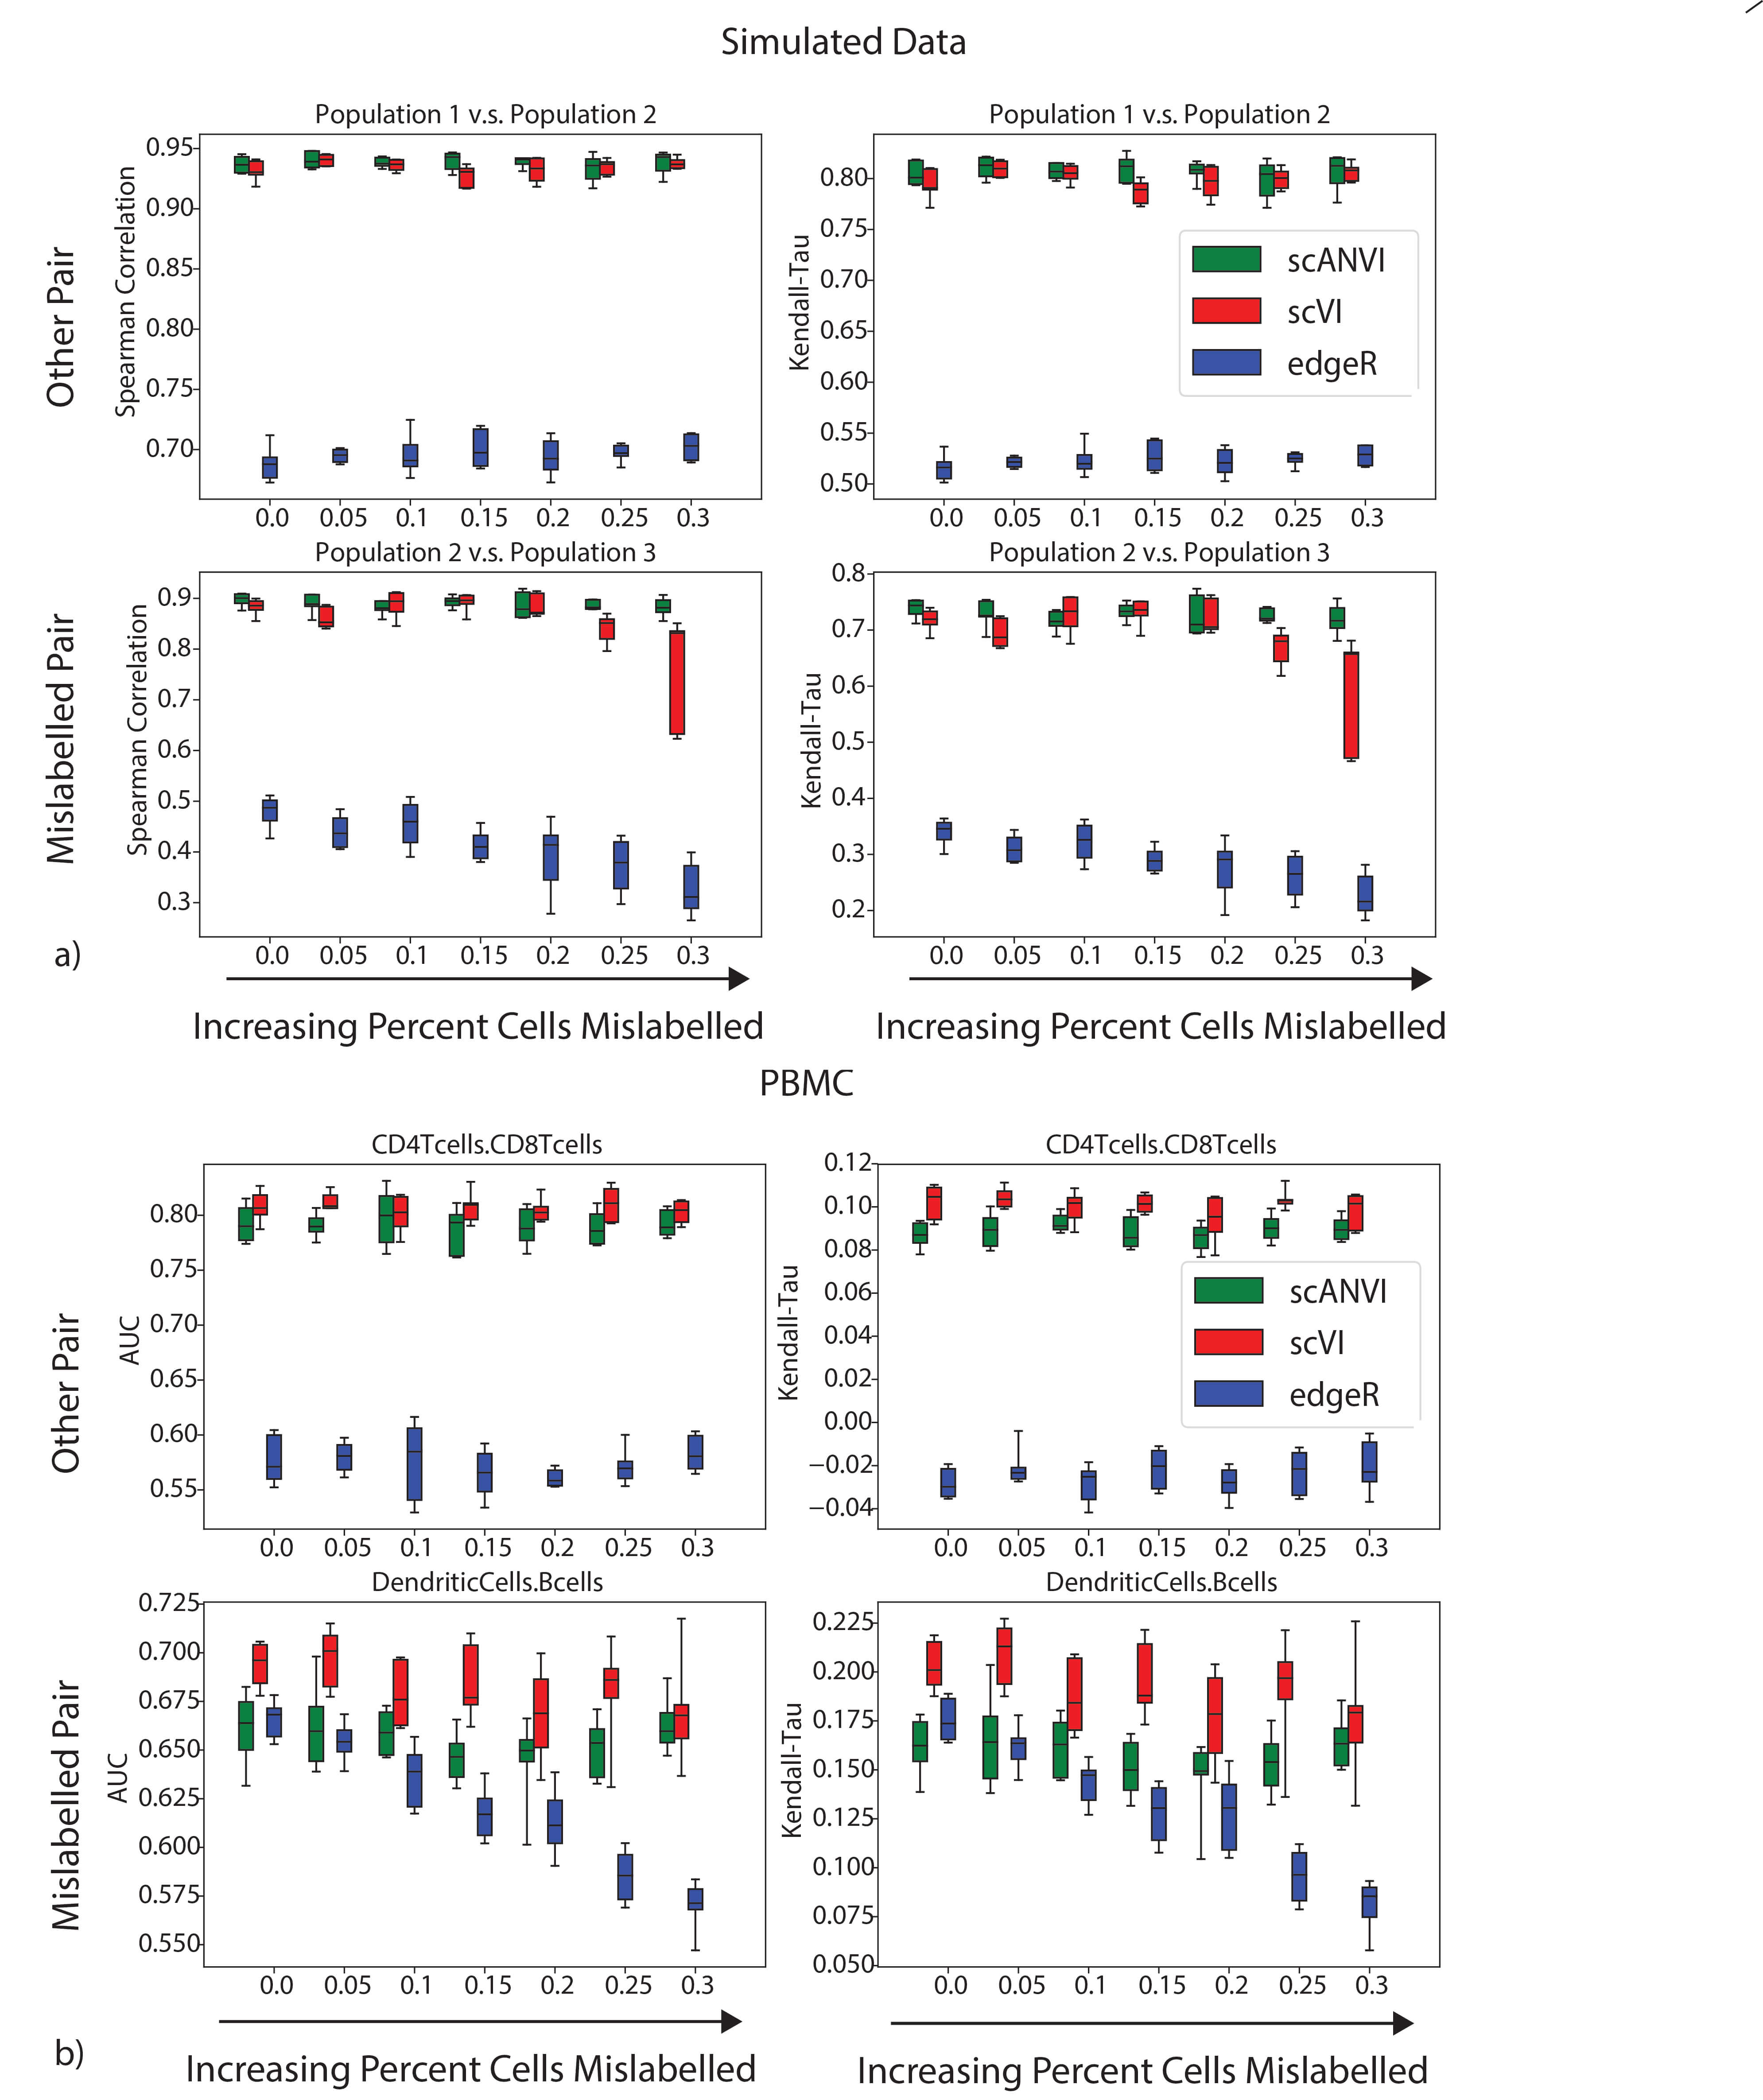
\includegraphics[width=0.9\textwidth]{figures/mislabelled.jpg}
\caption[Mislabeling experiment in differential expression]{Mislabeling experiment in differential expression with $(a)$ PBMC8K and PBMC68K datasets and $(b)$ SymSim simulated datasets. Within each panel: Top: differential expression results for the correctly labeled population pair (CD4 T cells - CD8 T cells in $(a)$ and 1-2 in $(b)$). Bottom: differential expression results for the mislabelled population pair (dendritic cells and B cells in $(a)$ and 2-3 in $(b)$). For all, x-axis represents the proportion of flipped labels. }
\label{scanviDE_mislabel}
\end{suppfigure}
% Combined Labels: 
% \caption

\begin{suppfigure}[H]
\centering
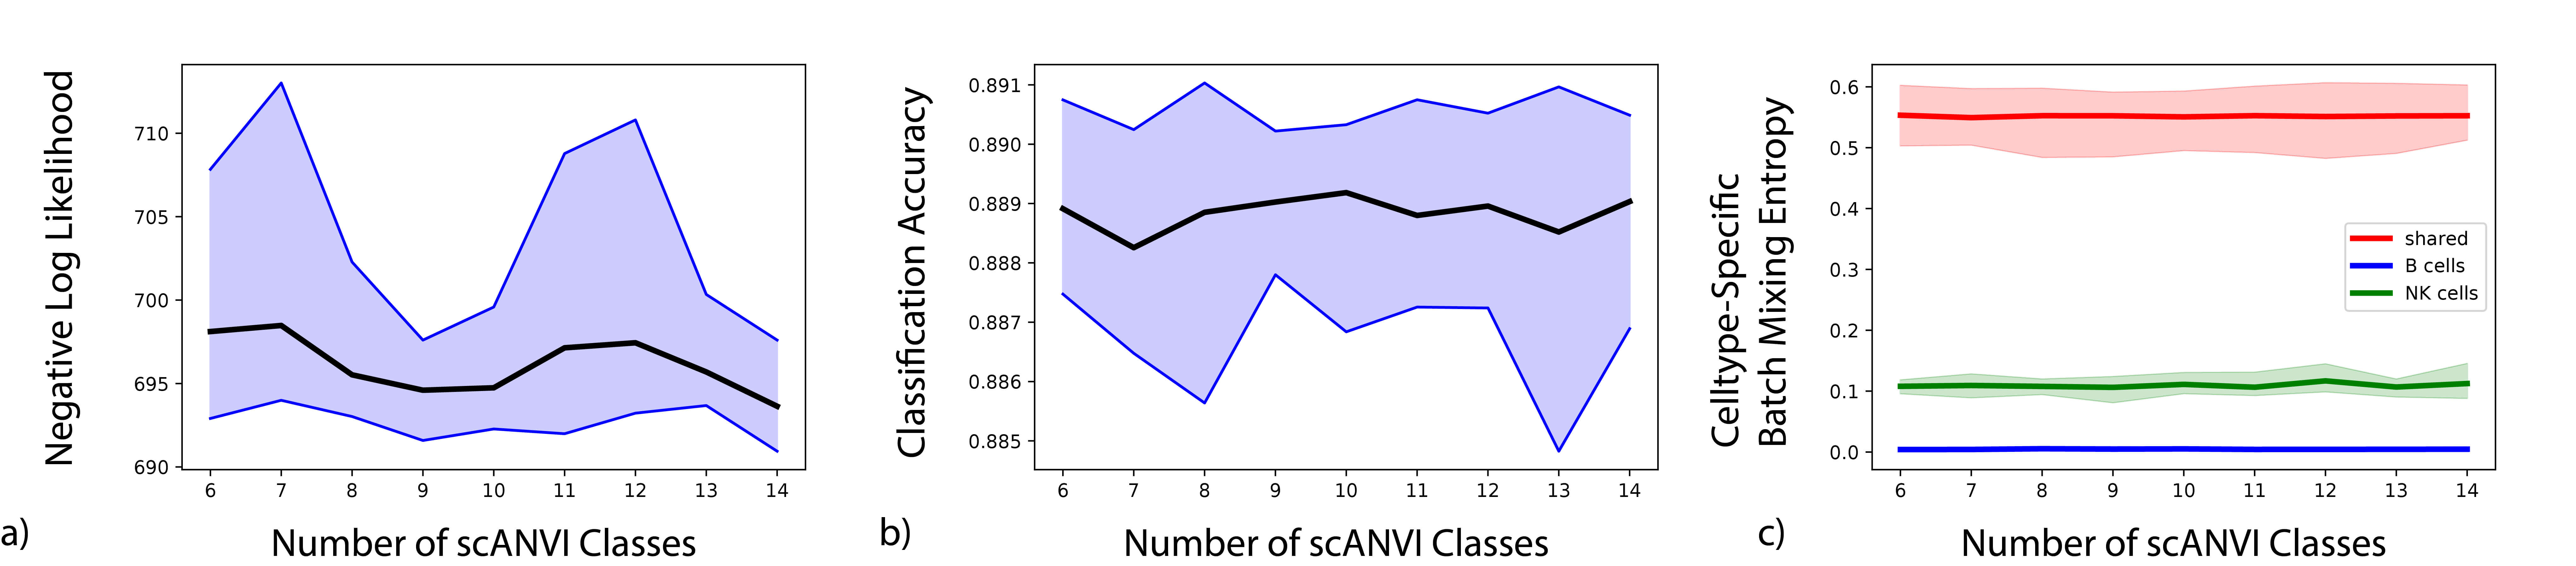
\includegraphics[width=\textwidth]{figures/Nclasses.jpg}
\caption[The effect of the choice of number of classes on the scANVI model]{The effect of the choice of number of classes on the scANVI model likelihood $(a)$, classification accuracy $(b)$ and entropy of batch mixing $(c)$. We trained scANVI using PBMC8K as the labelled dataset, and varied the number of classes in scANVI from 6(true number of labelled cell types) to 14. The thicker line show the mean of 9 replicates, while the colored shading show the 95\% confidence interval. We used a subsampled PBMC8K-CITE dataset, where NK cells are removed from the PBMC8K dataset and B cells are removed from the PBMC-CITE dataset. As we expect, the two unique dataset have low mixing in $(c)$ while the other cell types have high mixing. Although there is no labelled B cells, scANVI does not cluster B cells from the PBMC8K dataset with other cell types in PBMC-CITE. The three metrics we use to evaluate scANVI performance are minimally affected by the increase in the number of classes.  }
\label{scanviNclasses}
\end{suppfigure}

\begin{suppfigure}[H]
\centering
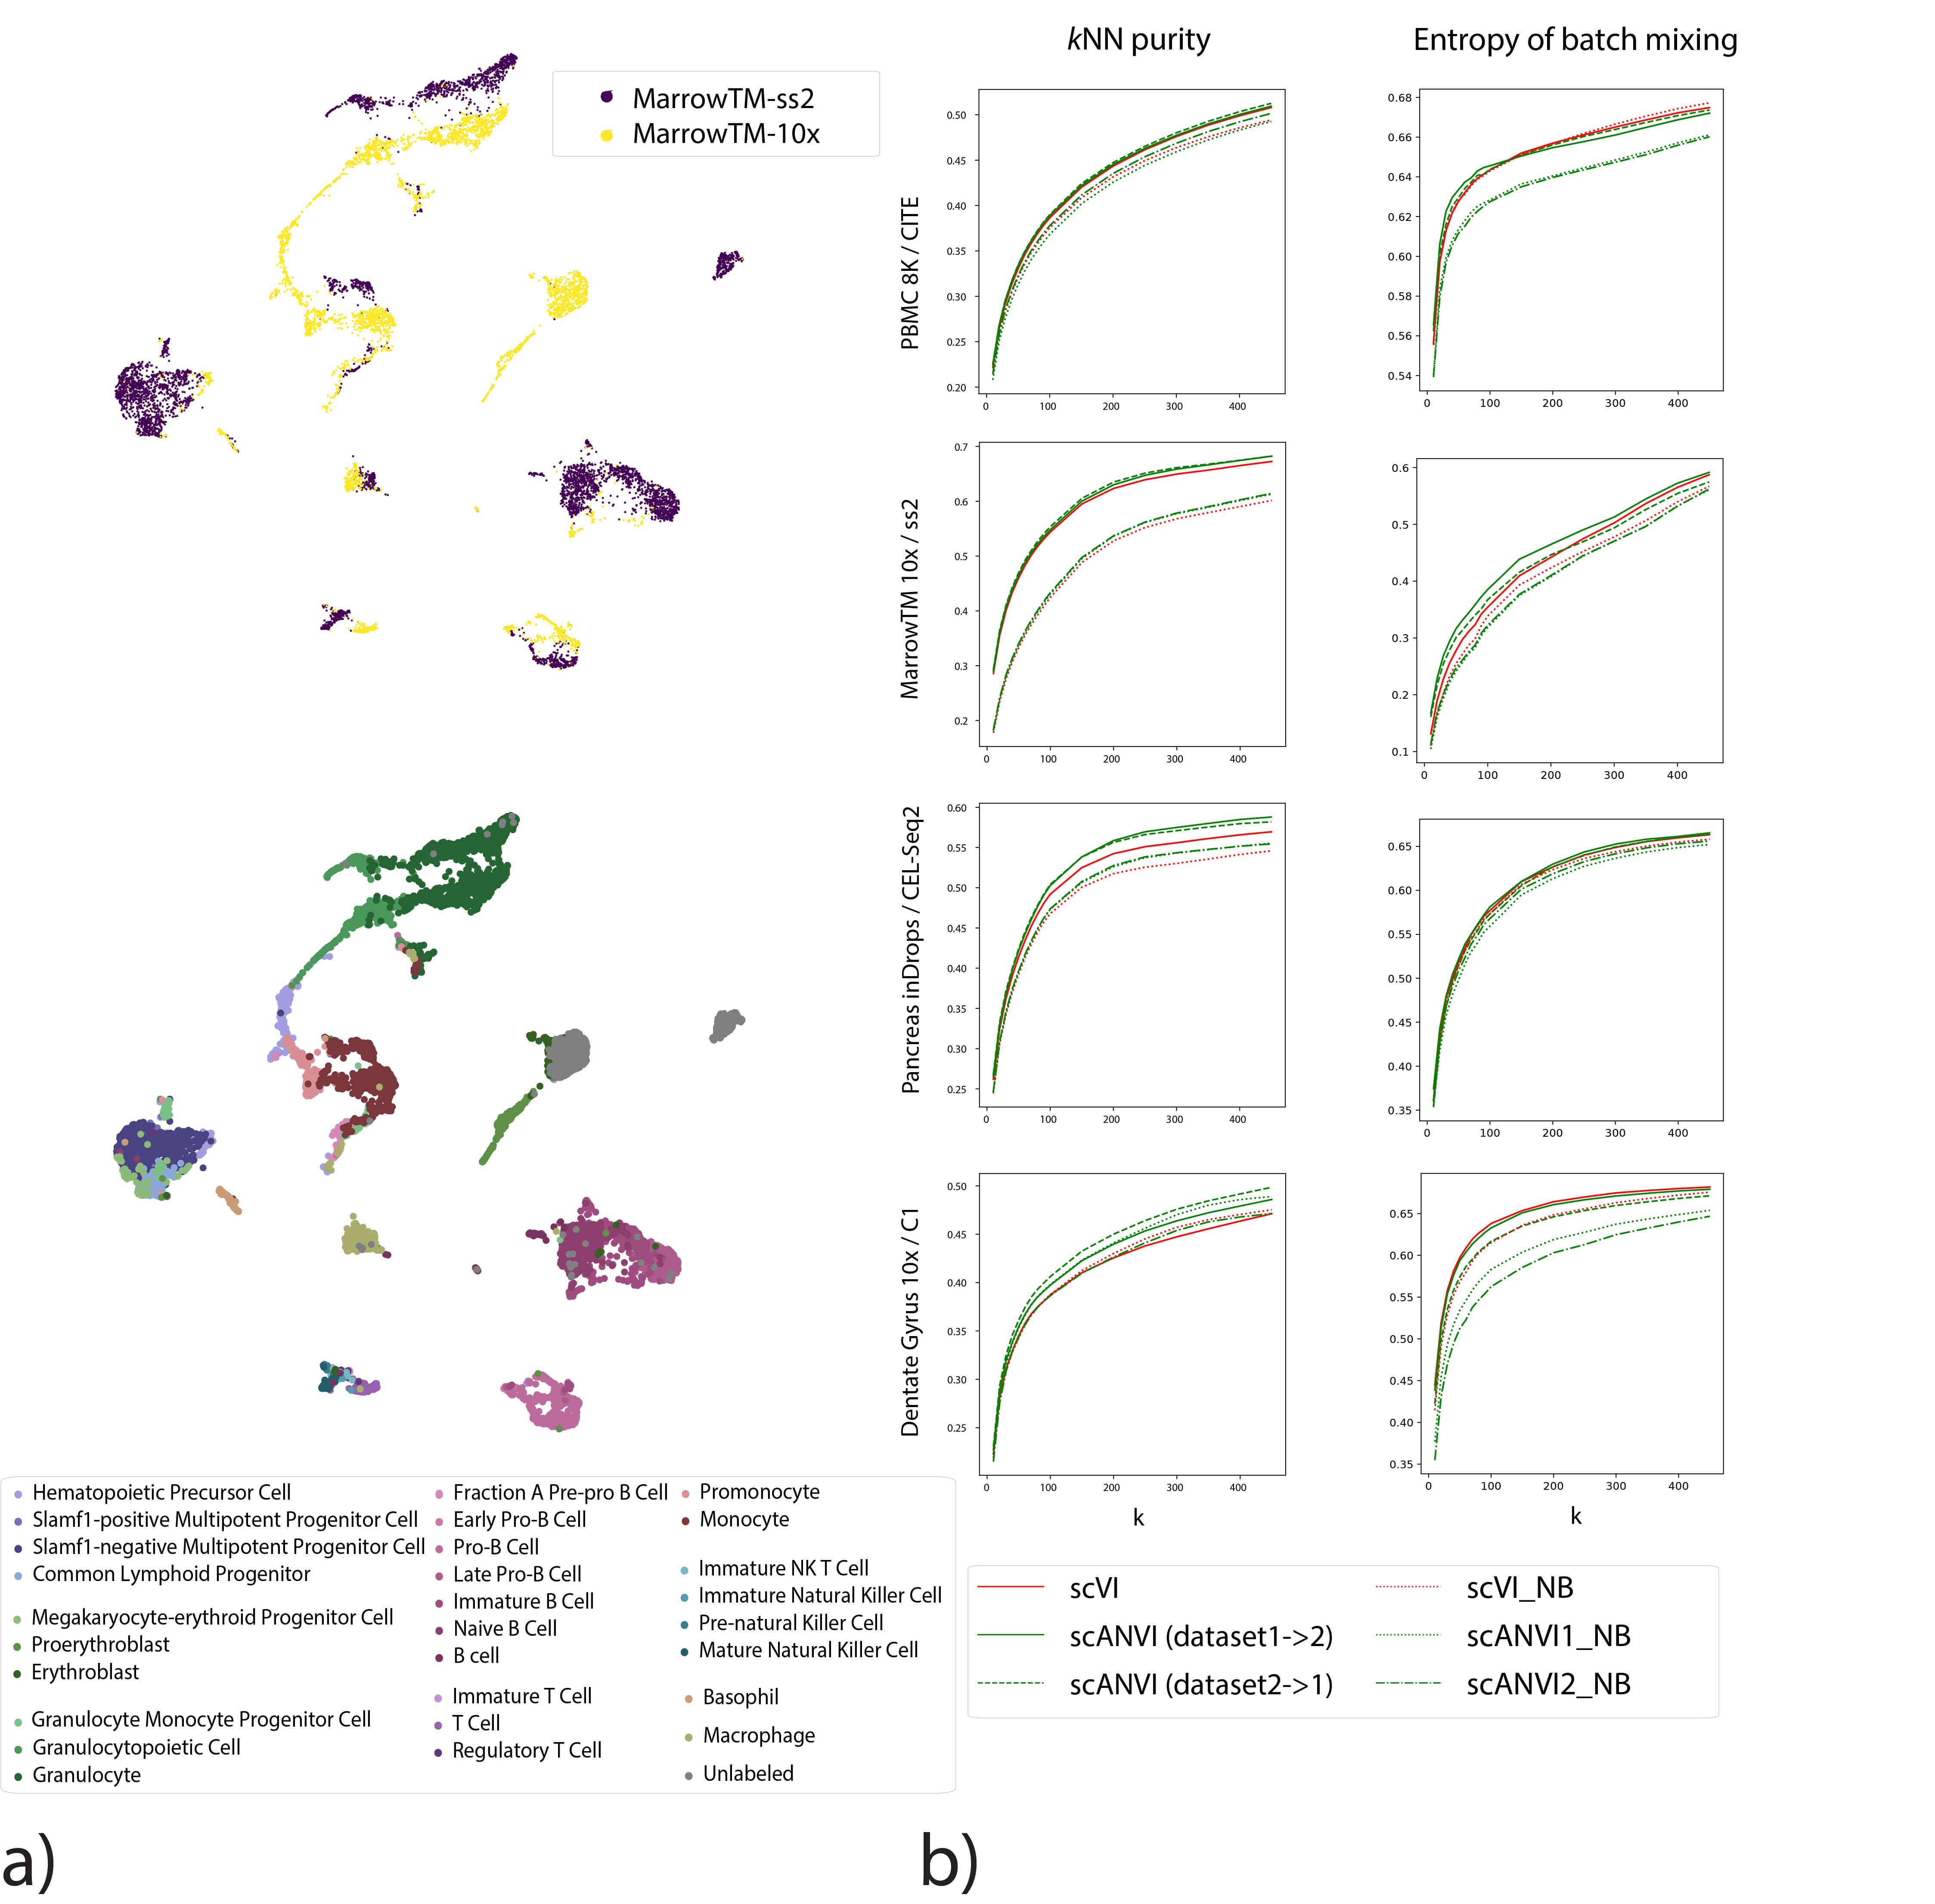
\includegraphics[width=\textwidth]{figures/ZINB_NB.jpg}
\caption[Performance of scVI and scANVI with a negative binomial (NB) distribution]{Performance of scVI and scANVI with a negative binomial (NB) distribution. $(a)$ UMAP plot of the MarrowTM pair using a NB distribution for scVI. $(b)$ Harmonization statistics and differences between regular scVI and NB version (scVI-NB). Dotted lines represent results using scVI-NB. }
\label{scanviZINB_NB}
\end{suppfigure}

\begin{suppfigure}[H]
\centering
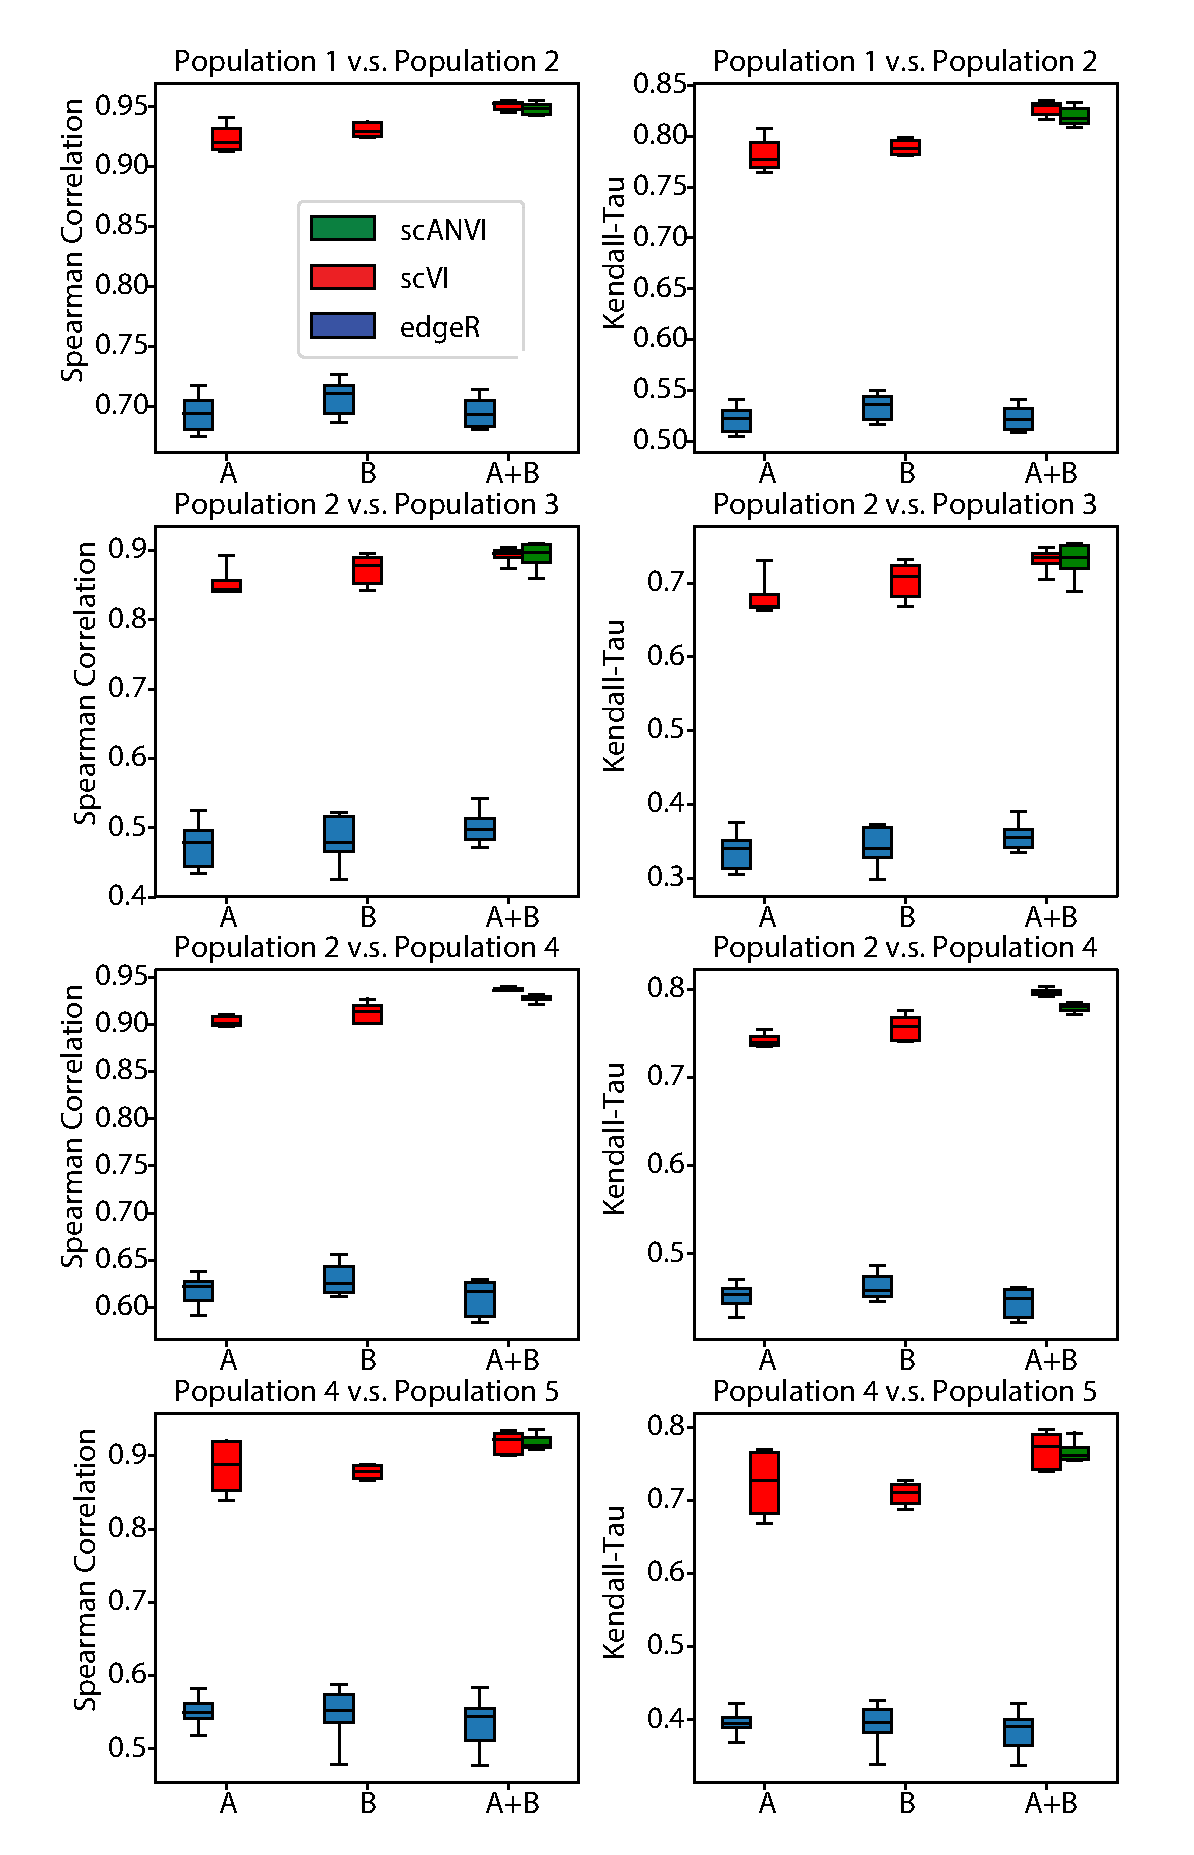
\includegraphics[width=0.7\textwidth]{figures/DE_NB.pdf}
\caption[Differential Expression with a negative binomial version of scVI]{Differential Expression with a negative binomial version of scVI. We report all metrics on all pairs of cell types using the simulated dataset previously analyzed as in Figure~\ref{scanvisimulations_panel}a.}
\label{scanviDE_NB}
\end{suppfigure}






